\section{Реализация}

Этапы реализации представлены в виде схемы (рис.~\ref{fig:fig1}). Разбиение на последовательные этапы позволяет контролировать процесс разработки и своевременно вносить коррективы~\cite{refl}.

\begin{figure}[htbp]
	\centering
	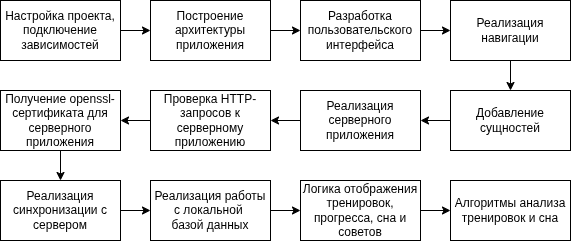
\includegraphics[width=1.0\textwidth]{images/diagrams/Этапы реализации.png}
	\caption{Схема этапов реализации приложения}
	\label{fig:fig1}
\end{figure}

\subsection{Подключение зависимостей}

Для написания приложения нужно добавить необходимые библиотеки в Gradle файле на уровне приложения. Разработка ведётся на языке Kotlin, поэтому используются его современные возможности~\cite{refa}. 
\begin{enumerate}
	\item Retrofit – это библиотека для работы с HTTP-запросами в Android-приложениях. Она используется для взаимодействия с собственным API, обеспечивая удобный и эффективный способ отправки запросов и обработки ответов. Конвертер Gson позволяет автоматически преобразовывать JSON-ответы от API в объекты Kotlin, что упрощает работу с данными. \cite{refg}\cite{refh}
	
	\item AndroidX Libraries предоставляет современные компоненты и инструменты для разработки Android-приложений, улучшая совместимость и функциональность. \cite{refg}
	
	\item Jetpack Compose для декларативной верстки экранов приложения. \cite{refg}
	
	\item Jetpack Navigation: обеспечивает удобный способ навигации между экранами приложения, упрощая управление компонентами и навигационными действиями. \cite{refh}
	
	\item Koin – это библиотека для внедрения зависимостей, которая упрощает создание и управление зависимостями в приложении, улучшая модульность и тестируемость кода.
	
	\item Room – это библиотека для работы с базой данных SQLite, предоставляющая удобный и безопасный способ хранения и управления данными в приложении. Благодаря ей будет происходить хранение информации о тренировках, упражнениях, сне и истории занятий.
\end{enumerate}

\subsection{Верстка экранов}

Все экраны приложения верстаются с помощью декларативного подхода Jetpack Compose. На этом этапе вынесены отдельно строковые и цветовые ресурсы, необходимые шрифты и векторные изображения для иконок. Для всех частей интерфейса используются стандартные UI-элементы Android SDK~\cite{refh}\cite{refb}.

Ниже представлены основные экраны приложения:
\begin{itemize}
    \item \textbf{Главный экран} (рис.~\ref{fig:main}) — отображает список доступных тренировок. Пока не начата работа с сетью, используются изображения-заглушки и тестовый текст.
    \item \textbf{Экран входа} (рис.~\ref{fig:signin}) — форма для авторизации пользователя.
    \item \textbf{Экран регистрации} (рис.~\ref{fig:signup}) — позволяет создать новый аккаунт.
    \item \textbf{Экран тренировки} (рис.~\ref{fig:training}) — показывает текущее упражнение, таймер и кнопки управления.
    \item \textbf{Экран профиля} (рис.~\ref{fig:profile}) — содержит информацию о пользователе и настройки.
\end{itemize}

Для похожих элементов UI вынесены одинаковые атрибуты в отдельный стиль для повторного использования. Также добавлена поддержка светлой и тёмной темы.

\begin{figure}[htbp]
    \centering
    \begin{minipage}{0.18\textwidth}
        \centering
        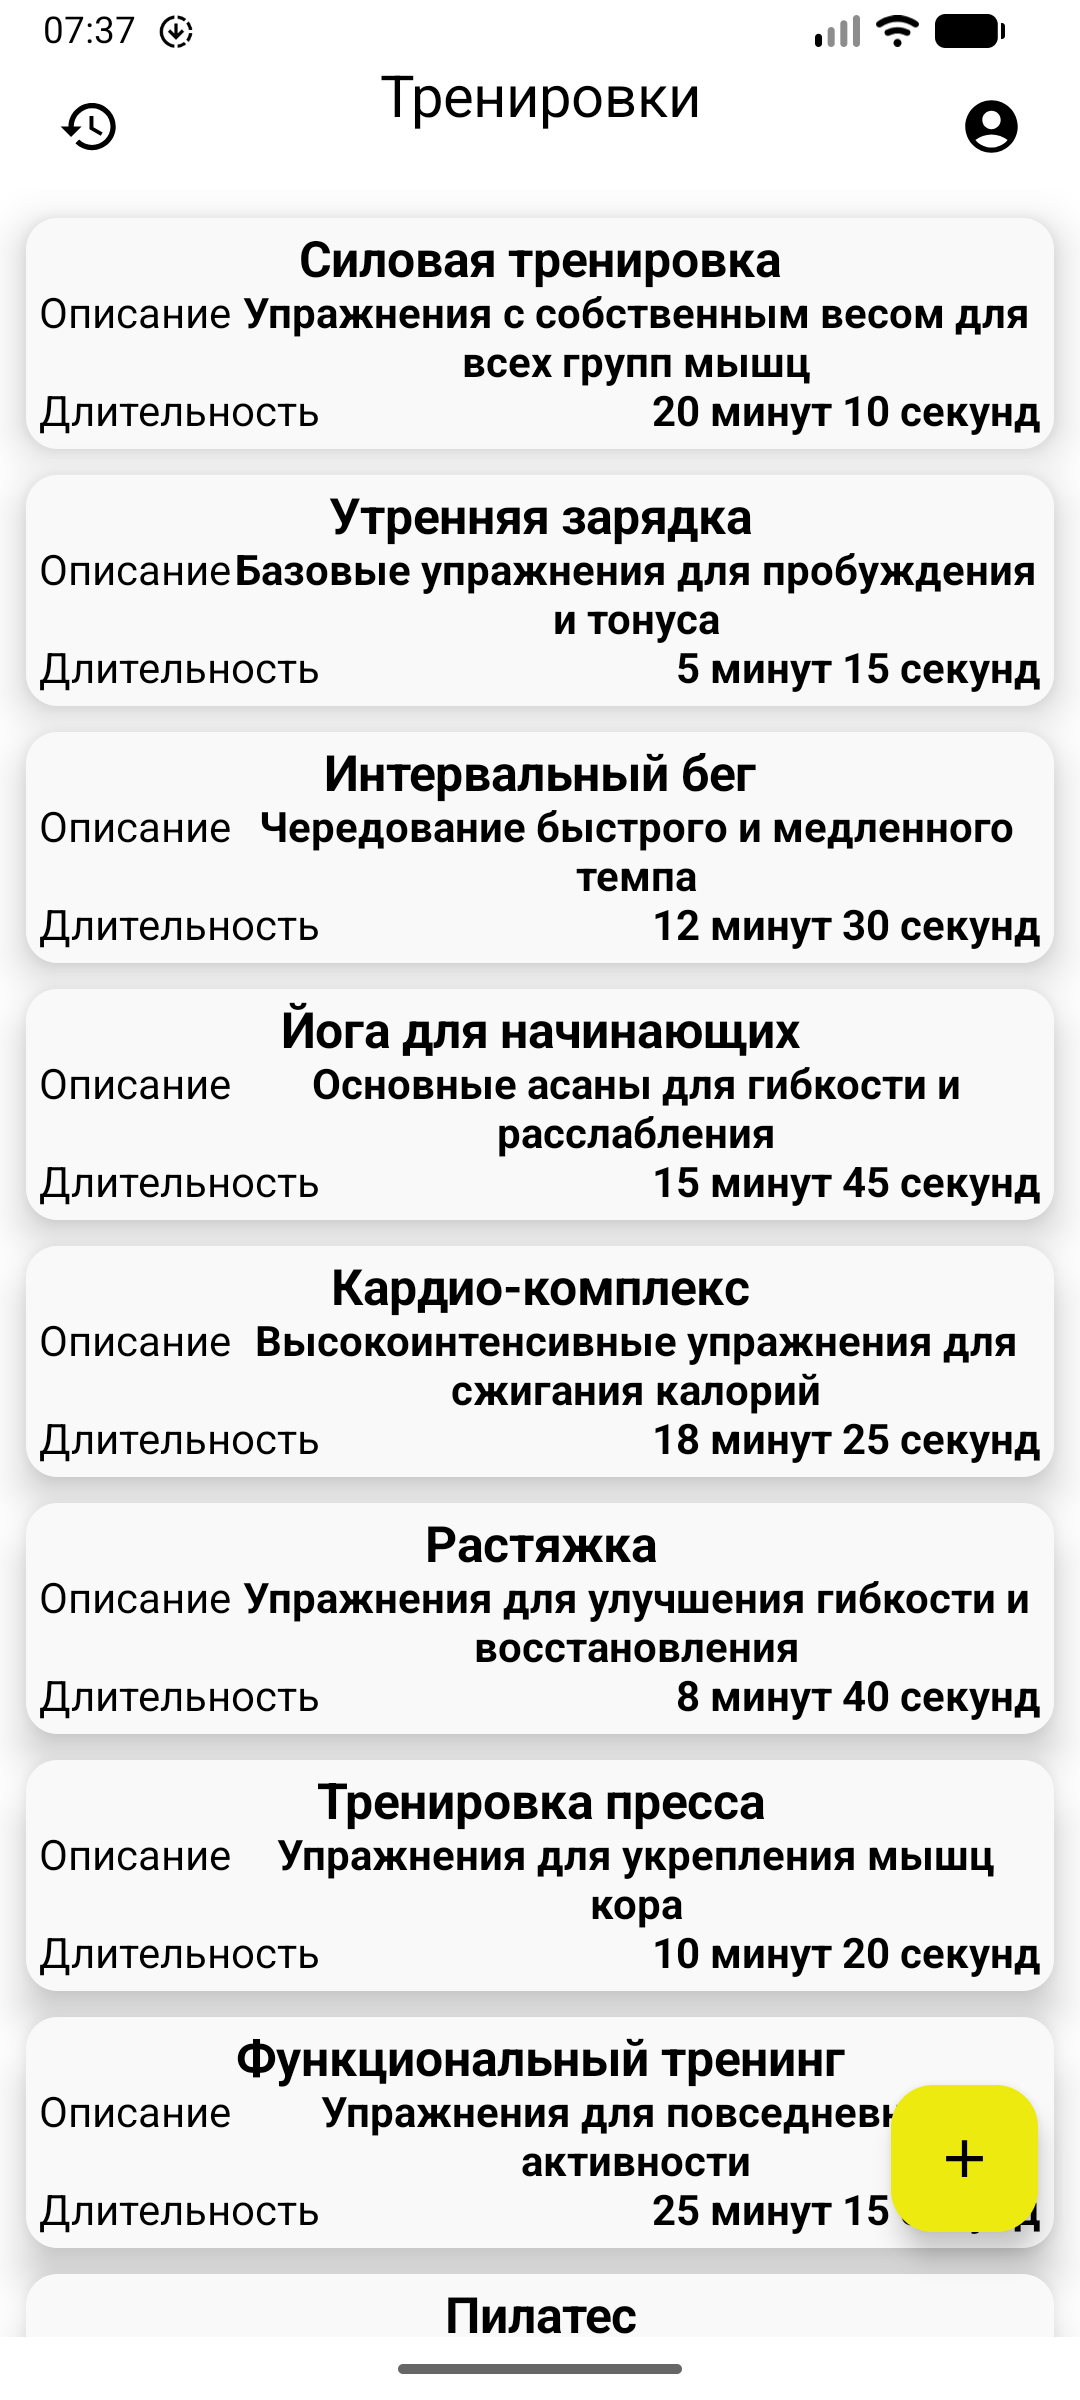
\includegraphics[width=\linewidth]{images/android_screens/main_screen.png}
        \captionof{figure}{Главный экран}
        \label{fig:main}
    \end{minipage}\hfill
    \begin{minipage}{0.18\textwidth}
        \centering
        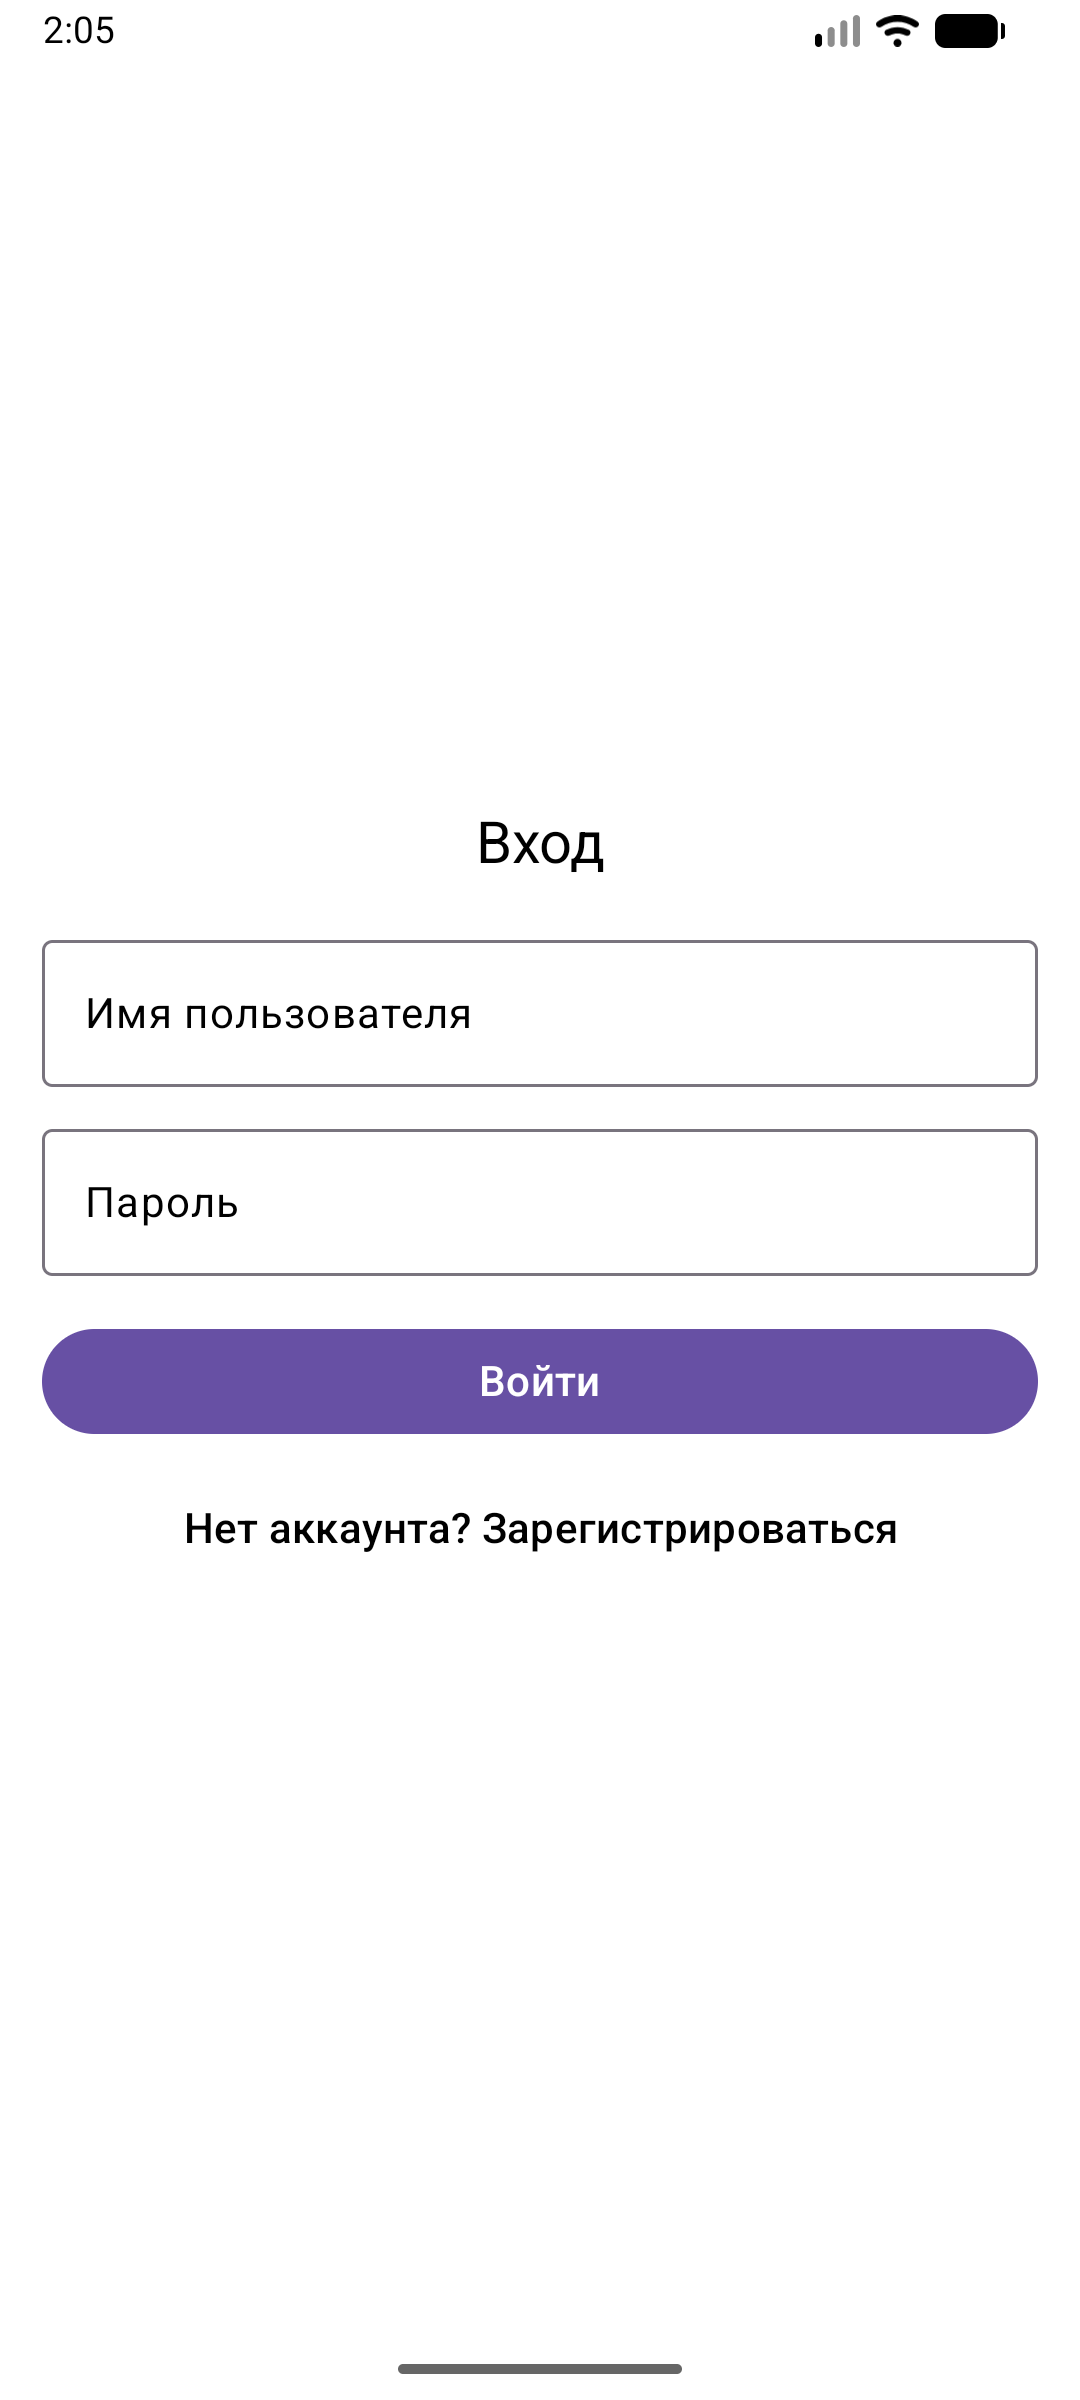
\includegraphics[width=\linewidth]{images/android_screens/sign_in.png}
        \captionof{figure}{Вход}
        \label{fig:signin}
    \end{minipage}\hfill
    \begin{minipage}{0.18\textwidth}
        \centering
        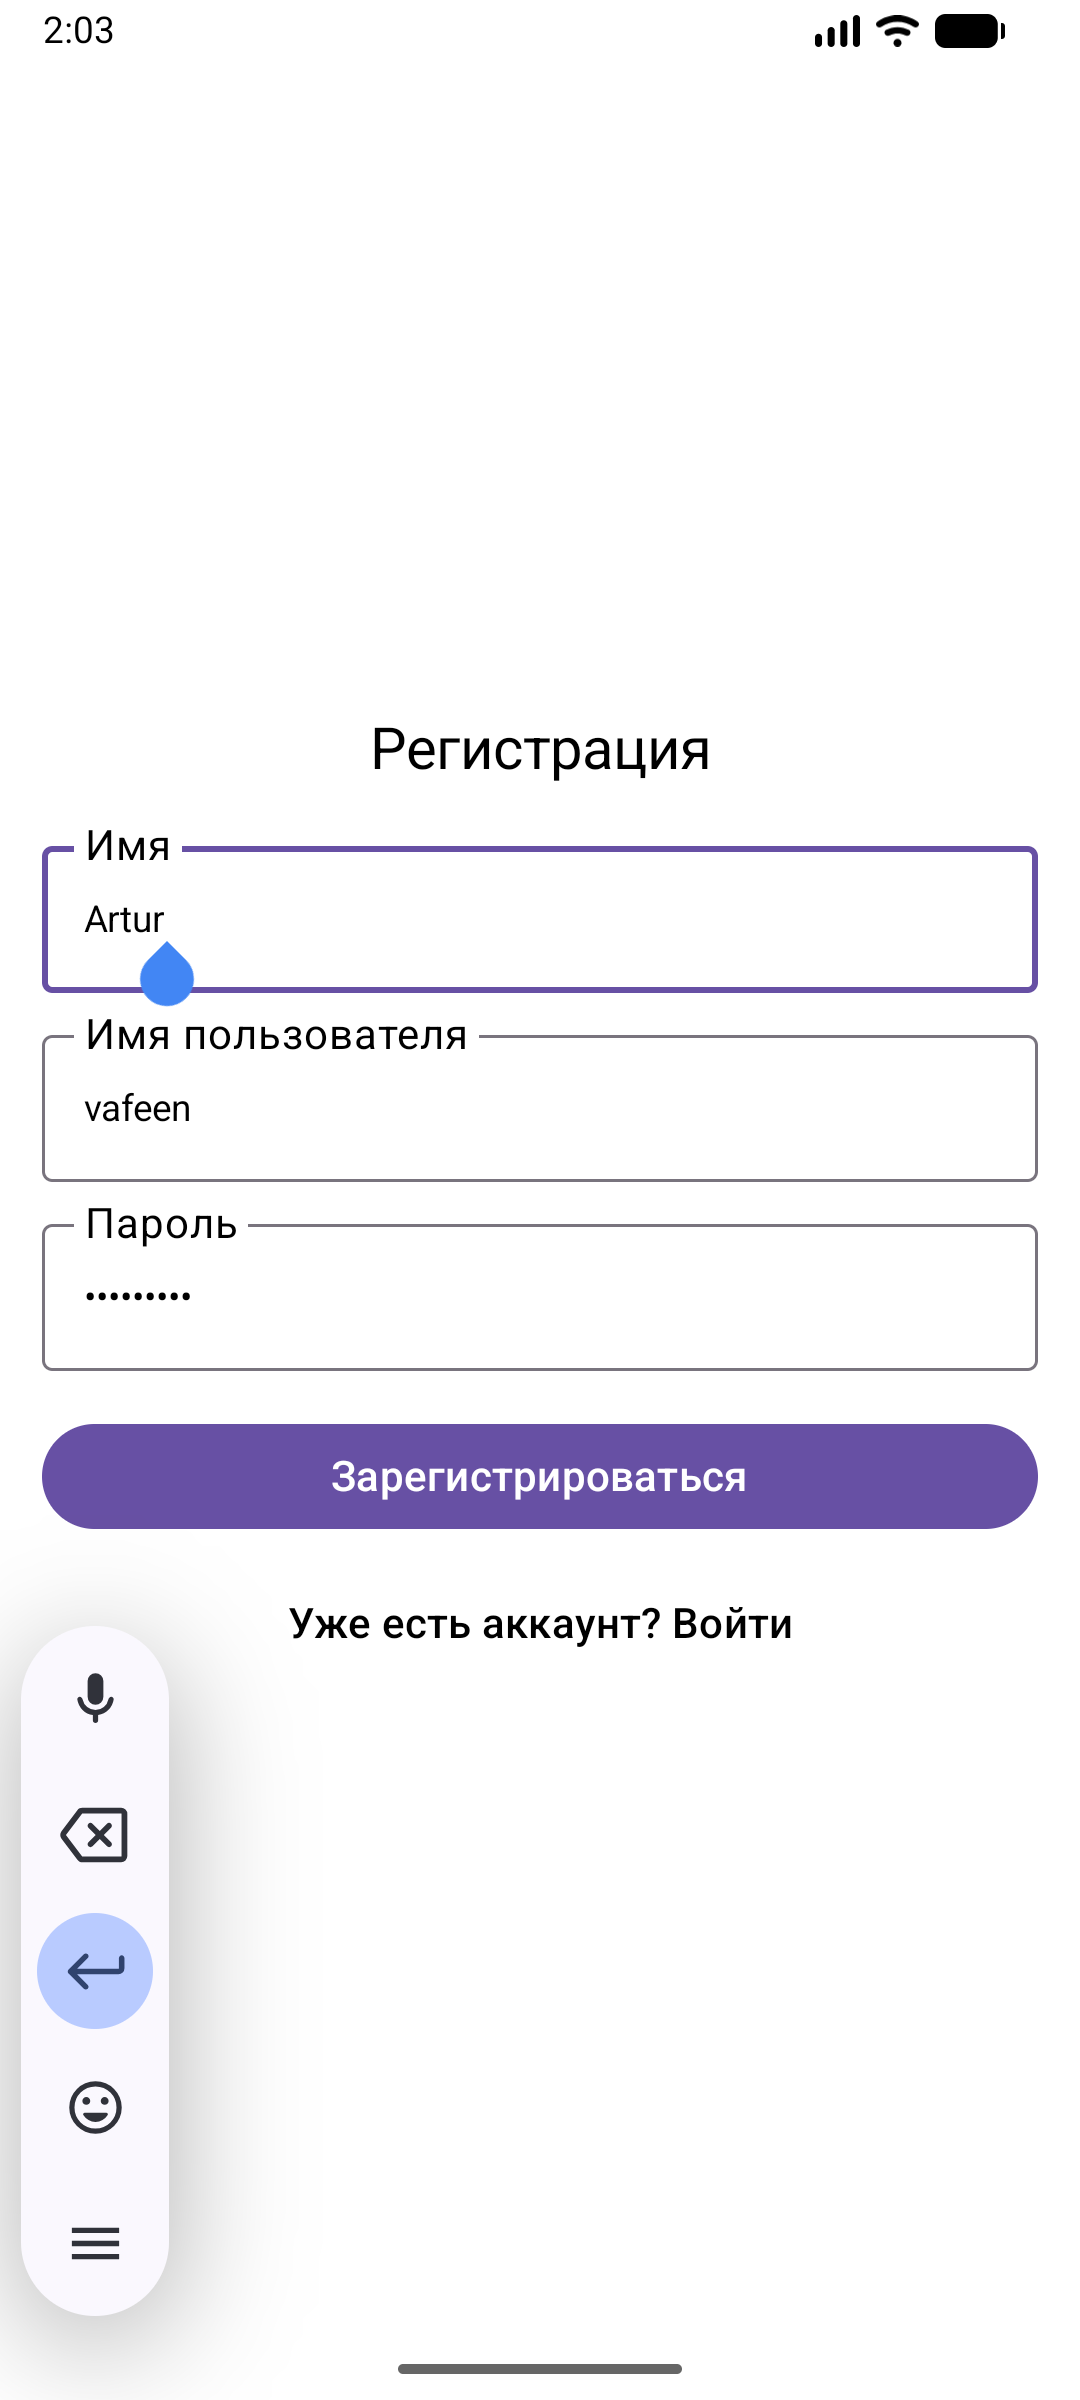
\includegraphics[width=\linewidth]{images/android_screens/sign_up.png}
        \captionof{figure}{Регистрация}
        \label{fig:signup}
    \end{minipage}\hfill
    \begin{minipage}{0.18\textwidth}
        \centering
        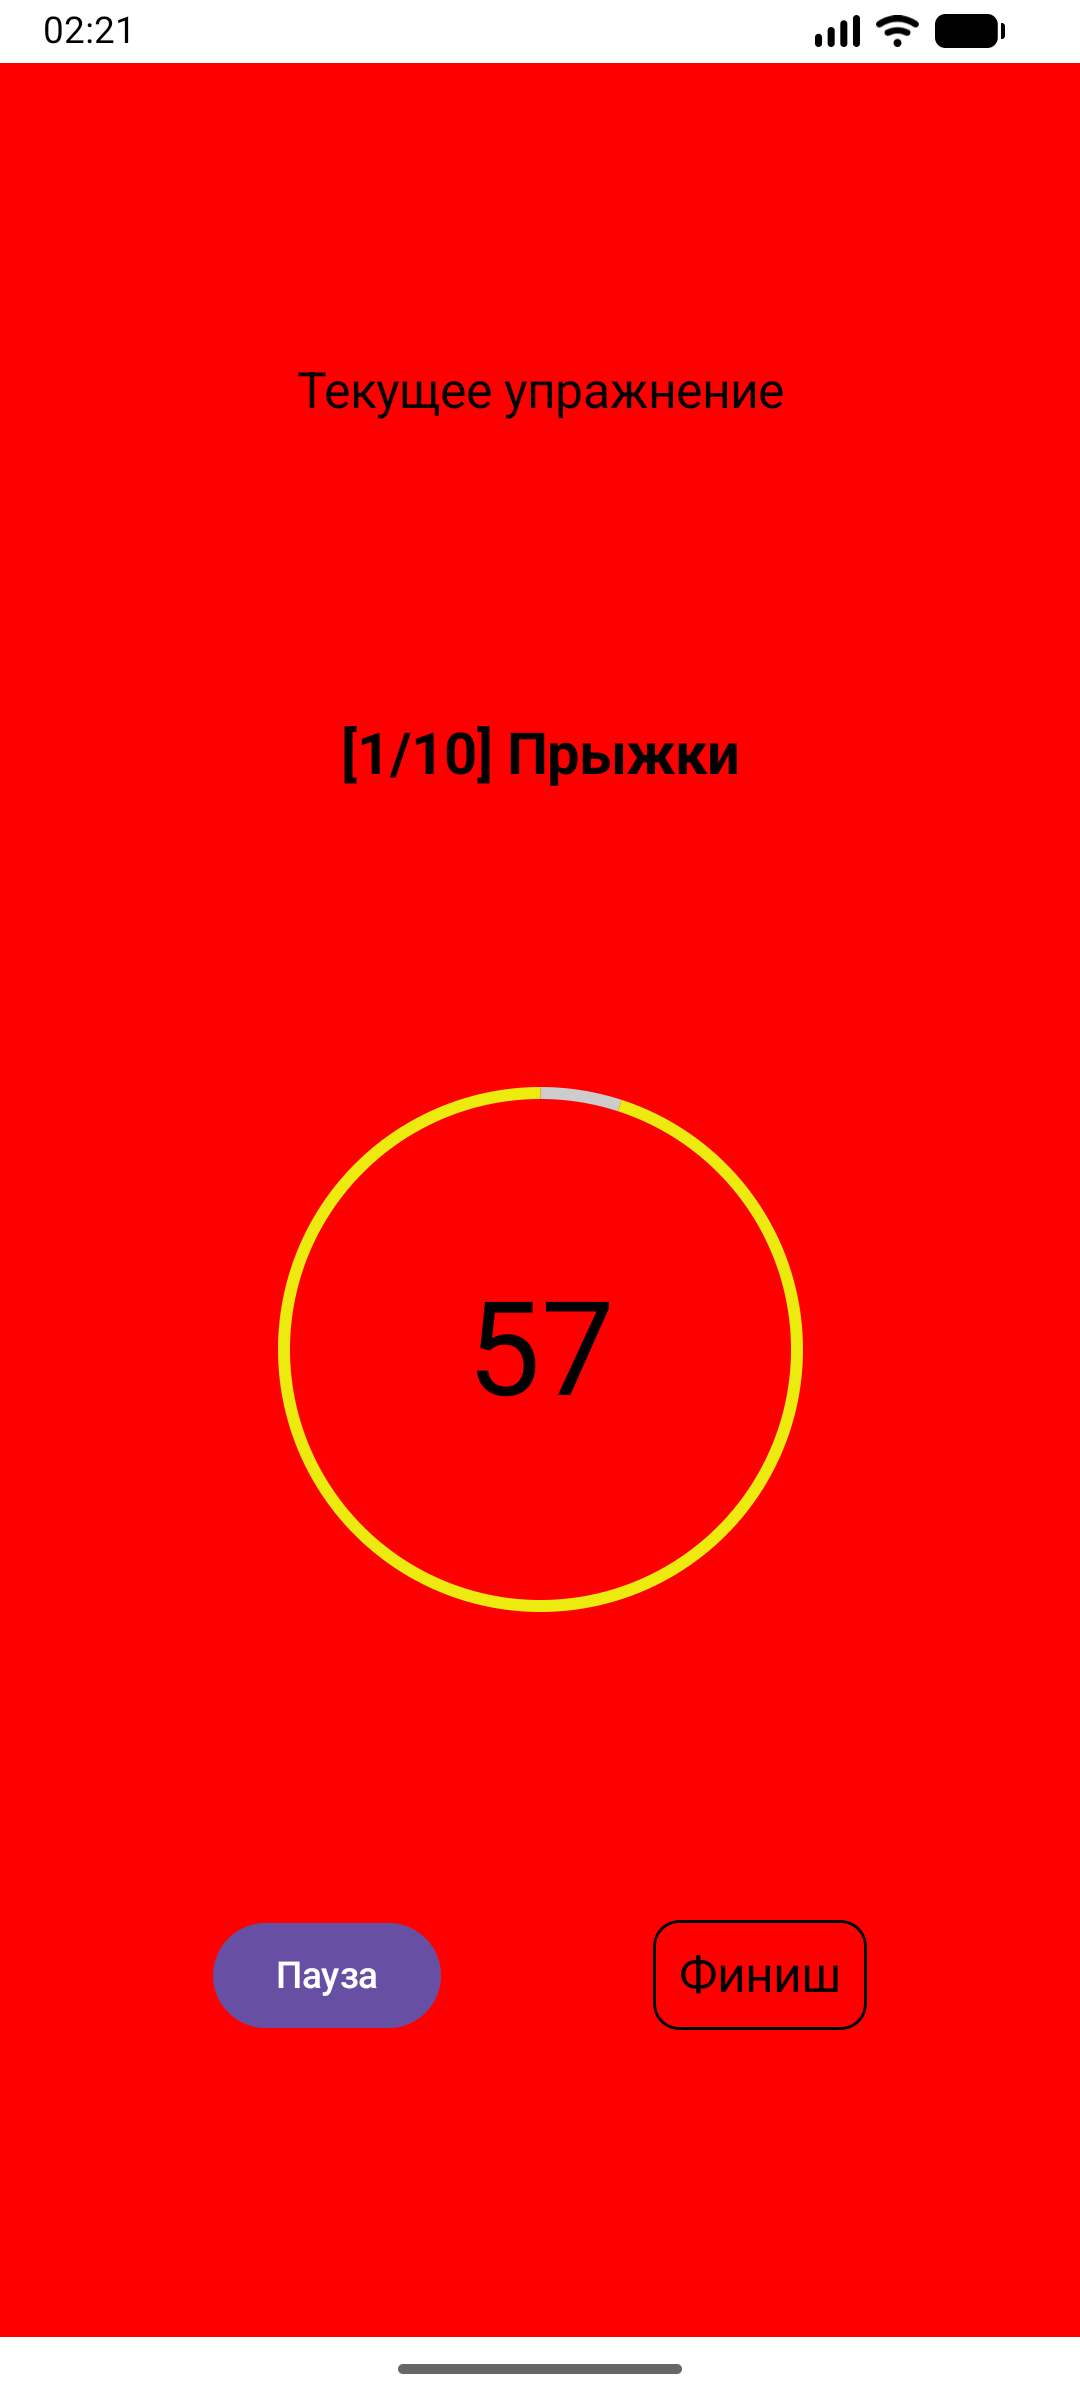
\includegraphics[width=\linewidth]{images/android_screens/training.png}
        \captionof{figure}{Тренировка}
        \label{fig:training}
    \end{minipage}\hfill
    \begin{minipage}{0.18\textwidth}
        \centering
        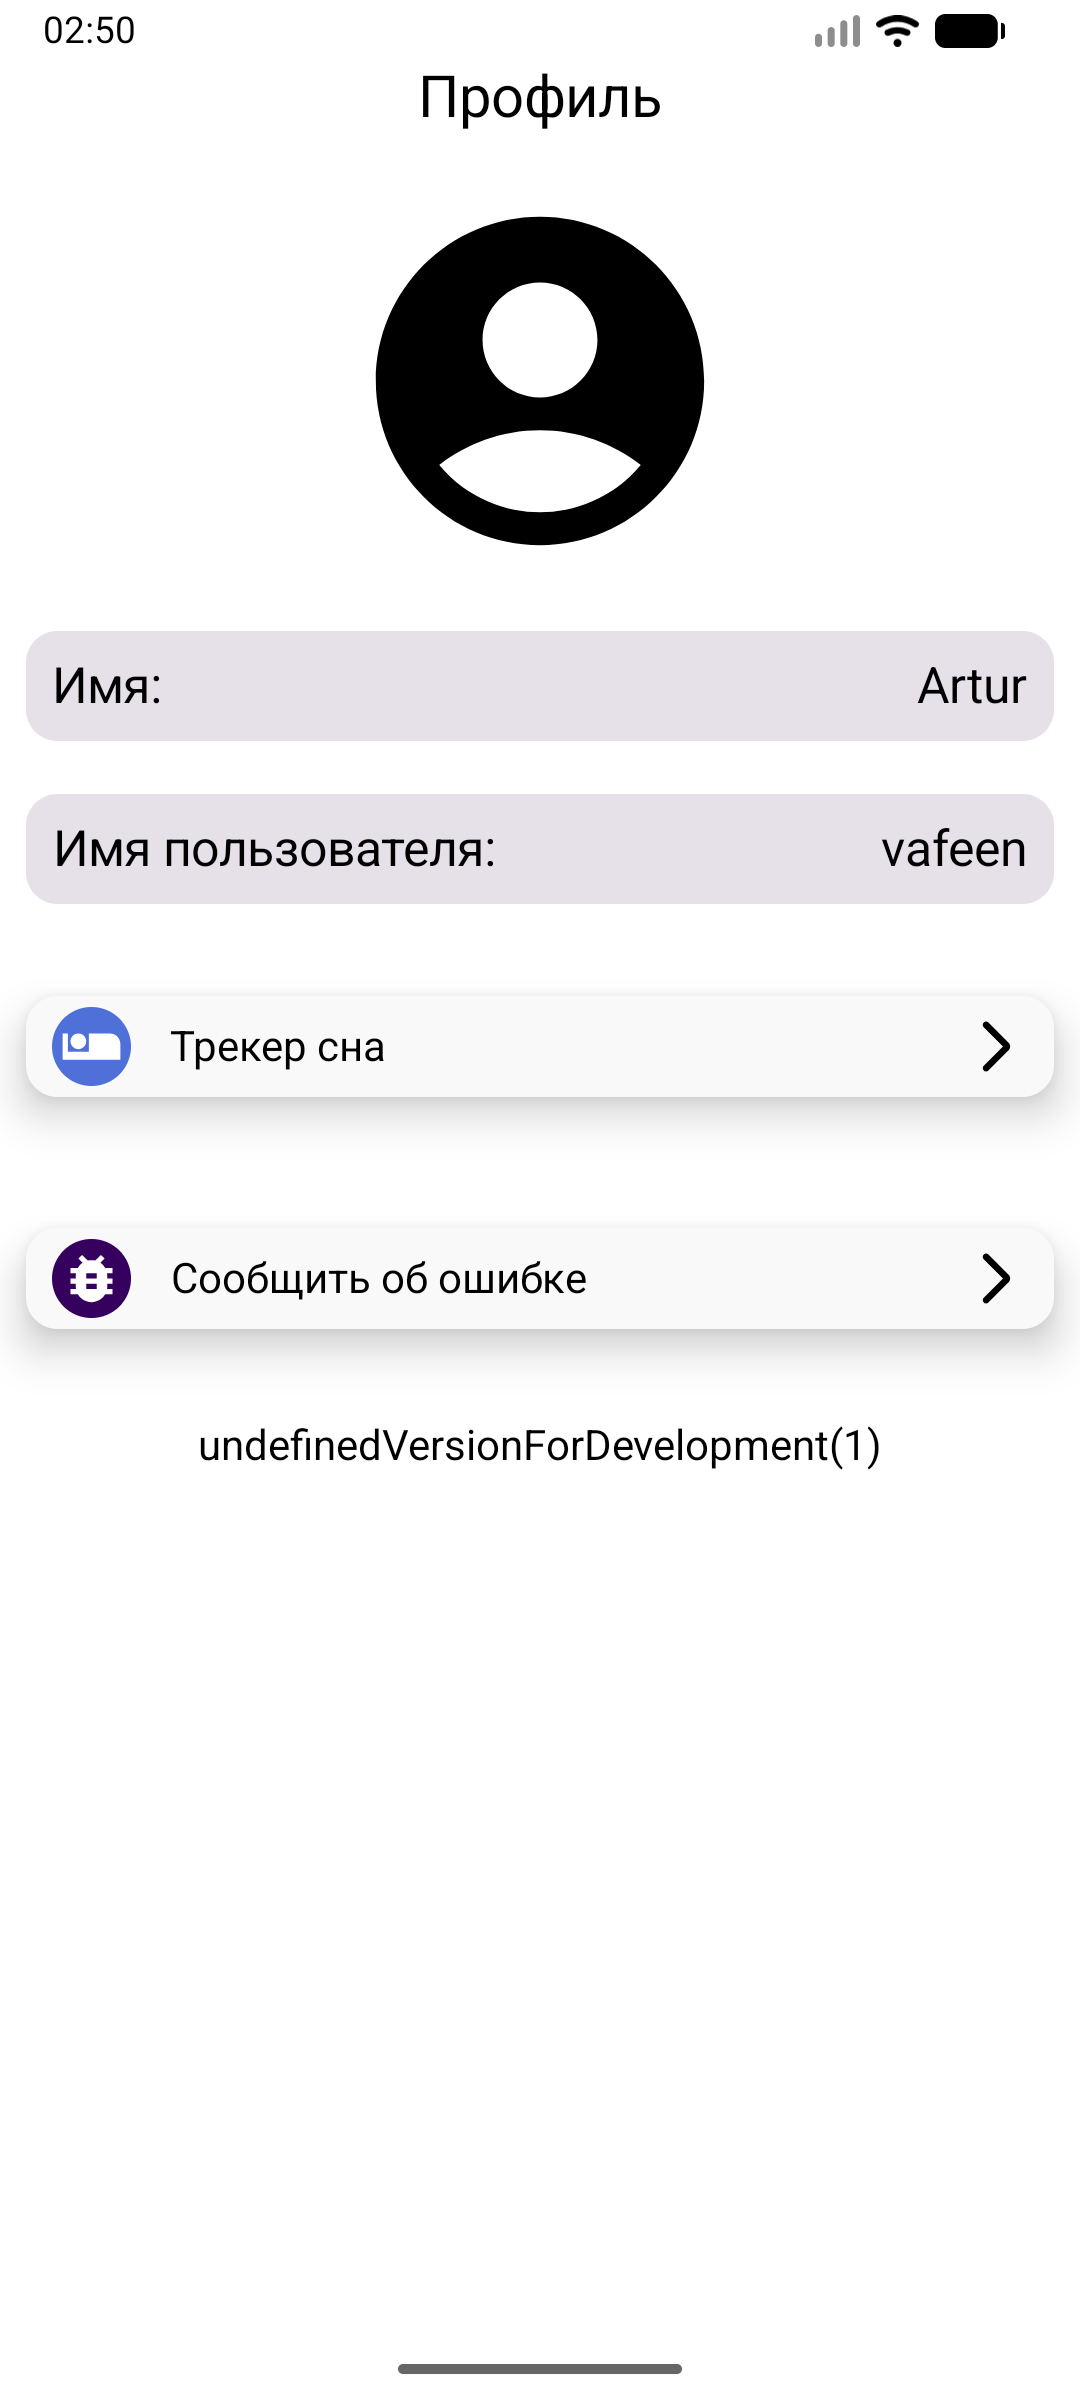
\includegraphics[width=\linewidth]{images/android_screens/profile_screen.png}
        \captionof{figure}{Профиль}
        \label{fig:profile}
    \end{minipage}
    \caption*{}
\end{figure}

Также ниже представлены экраны, связанные с процессом тренировки и статистикой. Описание упражнений опирается на анатомические и физиологические рекомендации~\cite{refk}:
\begin{itemize}
    \item \textbf{Экран перед тренировкой} (рис.~\ref{fig:before}) — отображает подготовительную информацию, рекомендации и кнопку старта.
    \item \textbf{Экран паузы} (рис.~\ref{fig:pause}) — появляется при приостановке тренировки, позволяет возобновить или завершить занятие.
    \item \textbf{Экран отдыха} (рис.~\ref{fig:rest}) — показывает таймер отдыха между подходами.
    \item \textbf{Экран истории} (рис.~\ref{fig:history}) — содержит список завершённых тренировок с датами и основными показателями.
    \item \textbf{Экран трекера сна} (рис.~\ref{fig:sleep}) — позволяет отслеживать продолжительность сна.
\end{itemize}

\begin{figure}[htbp]
    \centering
    \begin{minipage}{0.18\textwidth}
        \centering
        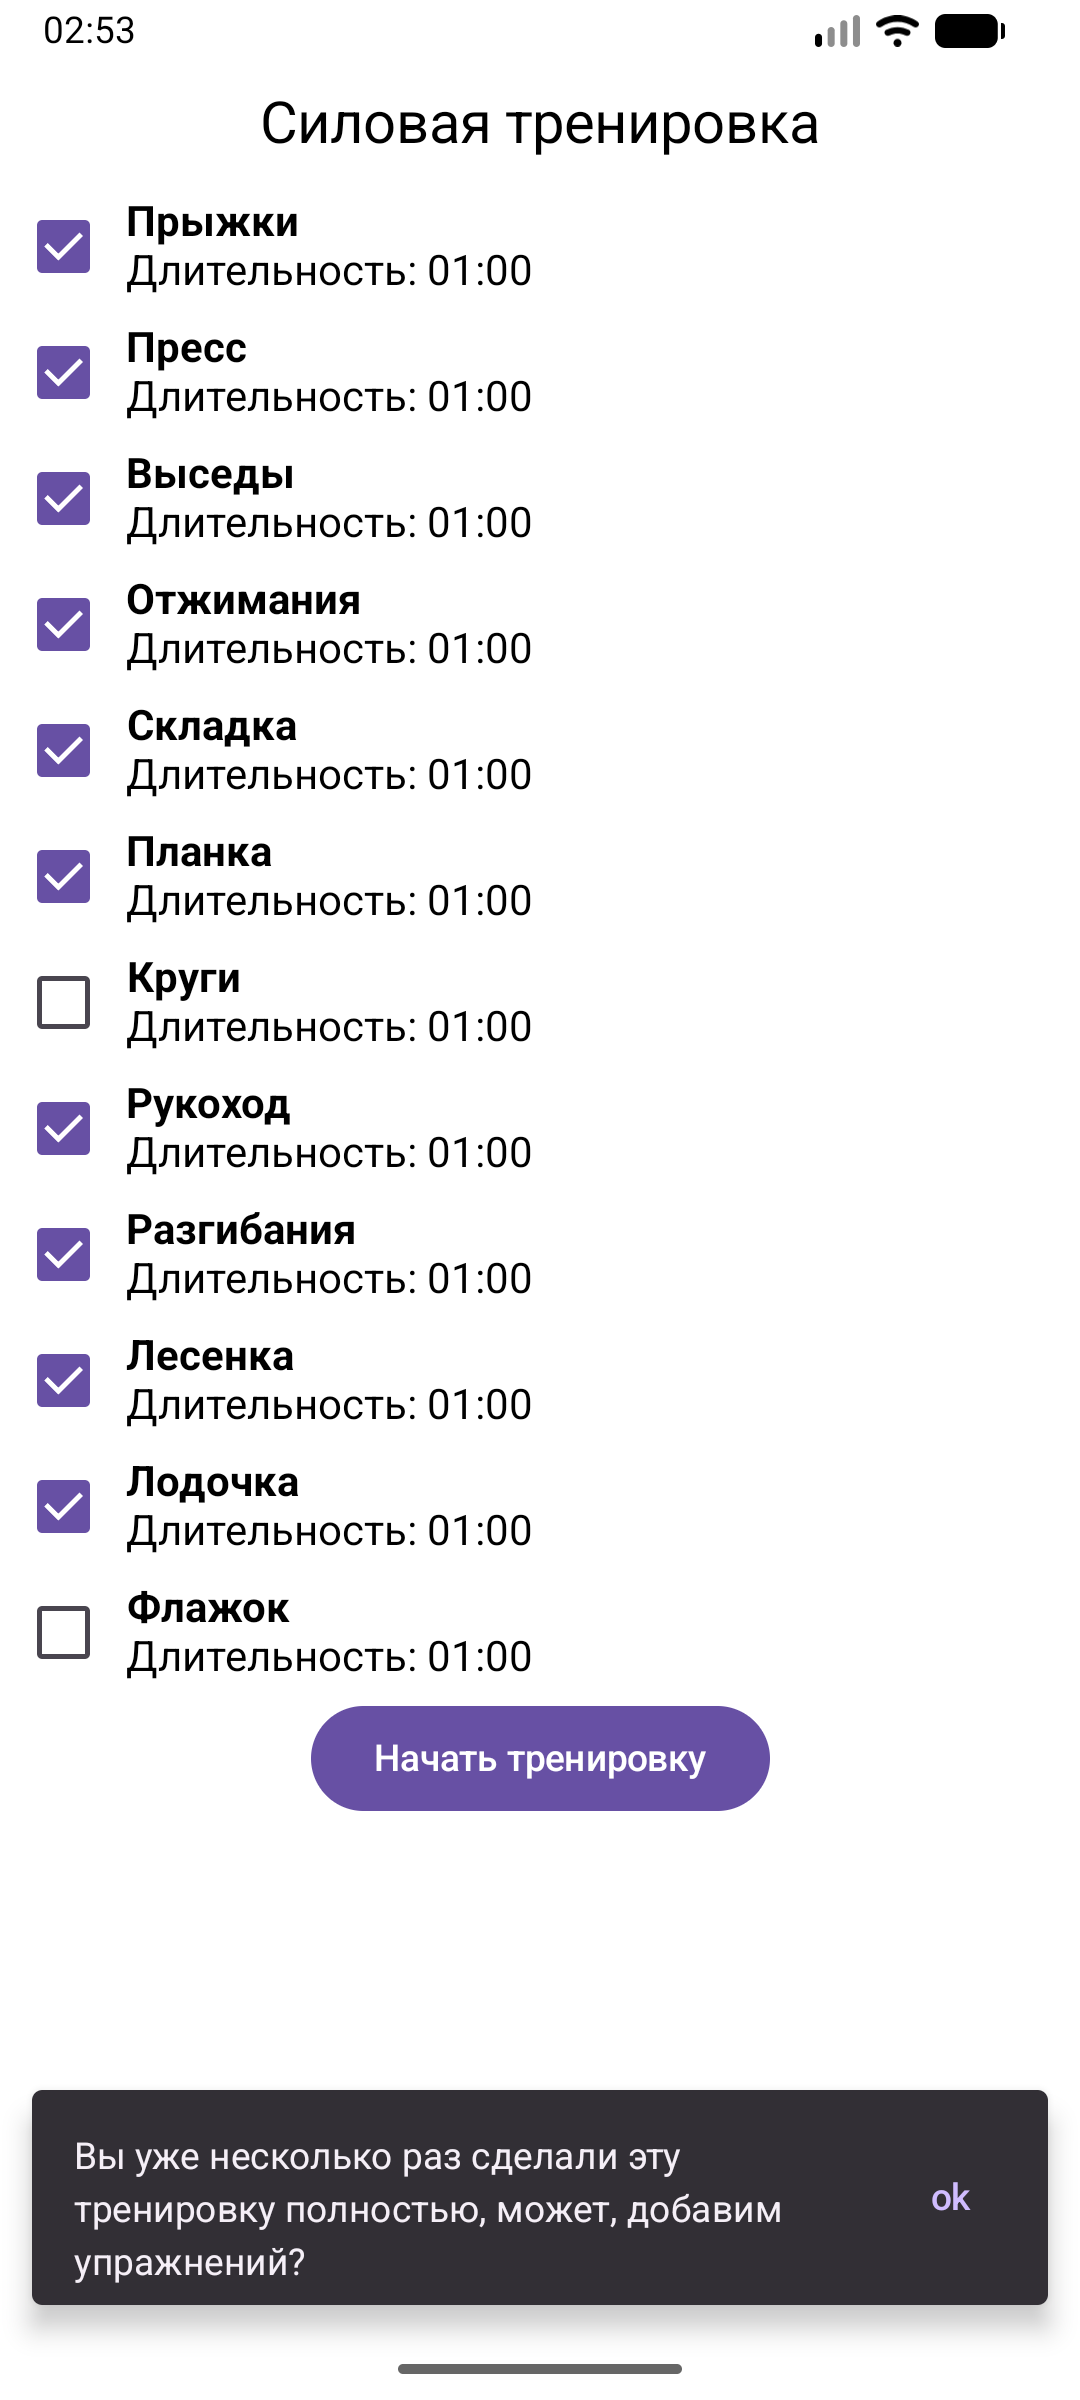
\includegraphics[width=\linewidth]{images/android_screens/before_training.png}
        \captionof{figure}{Перед тренировкой}
        \label{fig:before}
    \end{minipage}\hfill
    \begin{minipage}{0.18\textwidth}
        \centering
        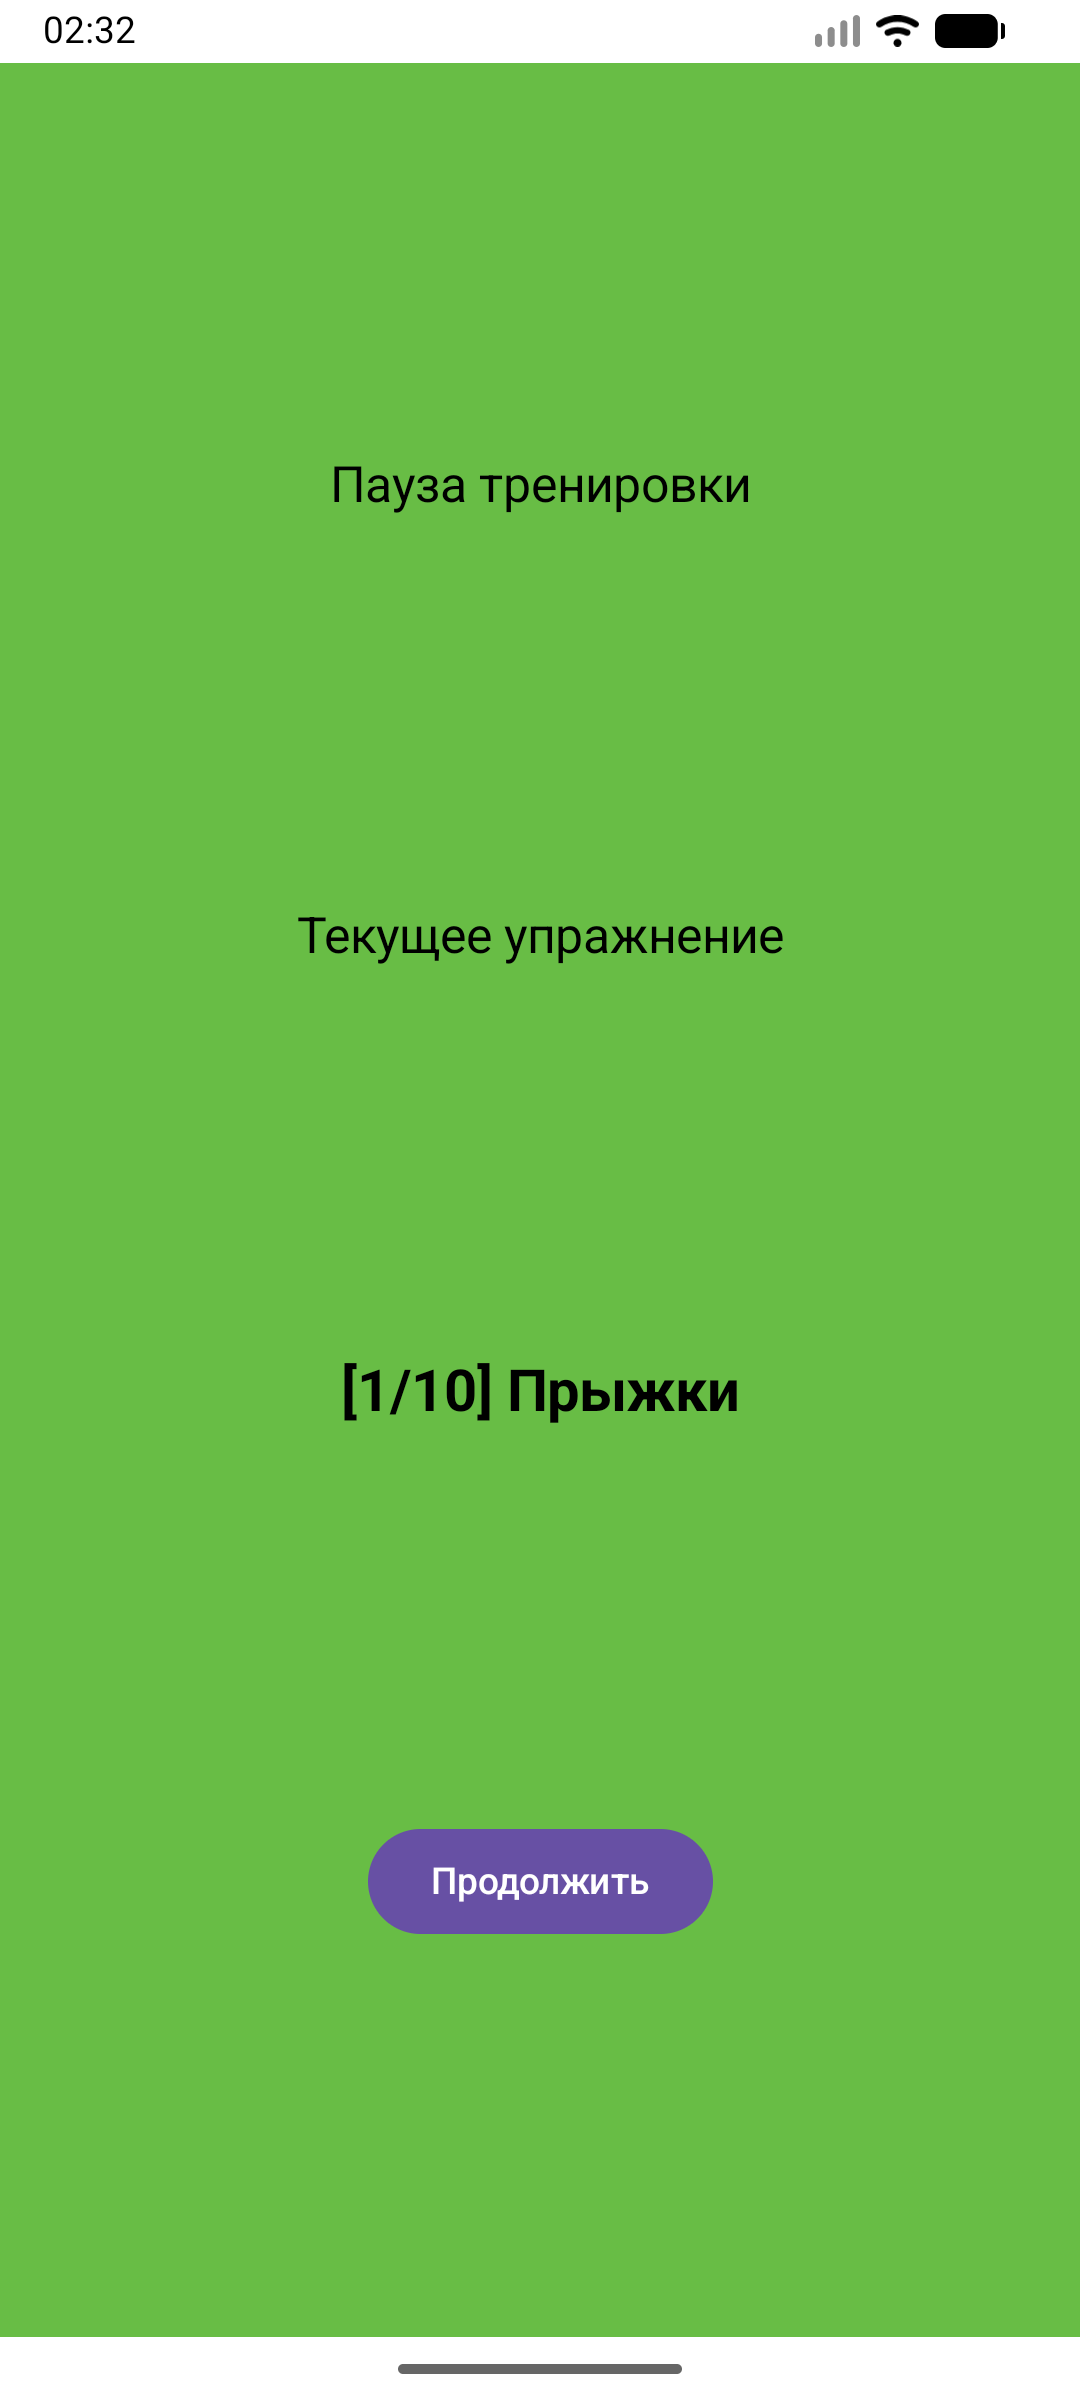
\includegraphics[width=\linewidth]{images/android_screens/pause.png}
        \captionof{figure}{Пауза}
        \label{fig:pause}
    \end{minipage}\hfill
    \begin{minipage}{0.18\textwidth}
        \centering
        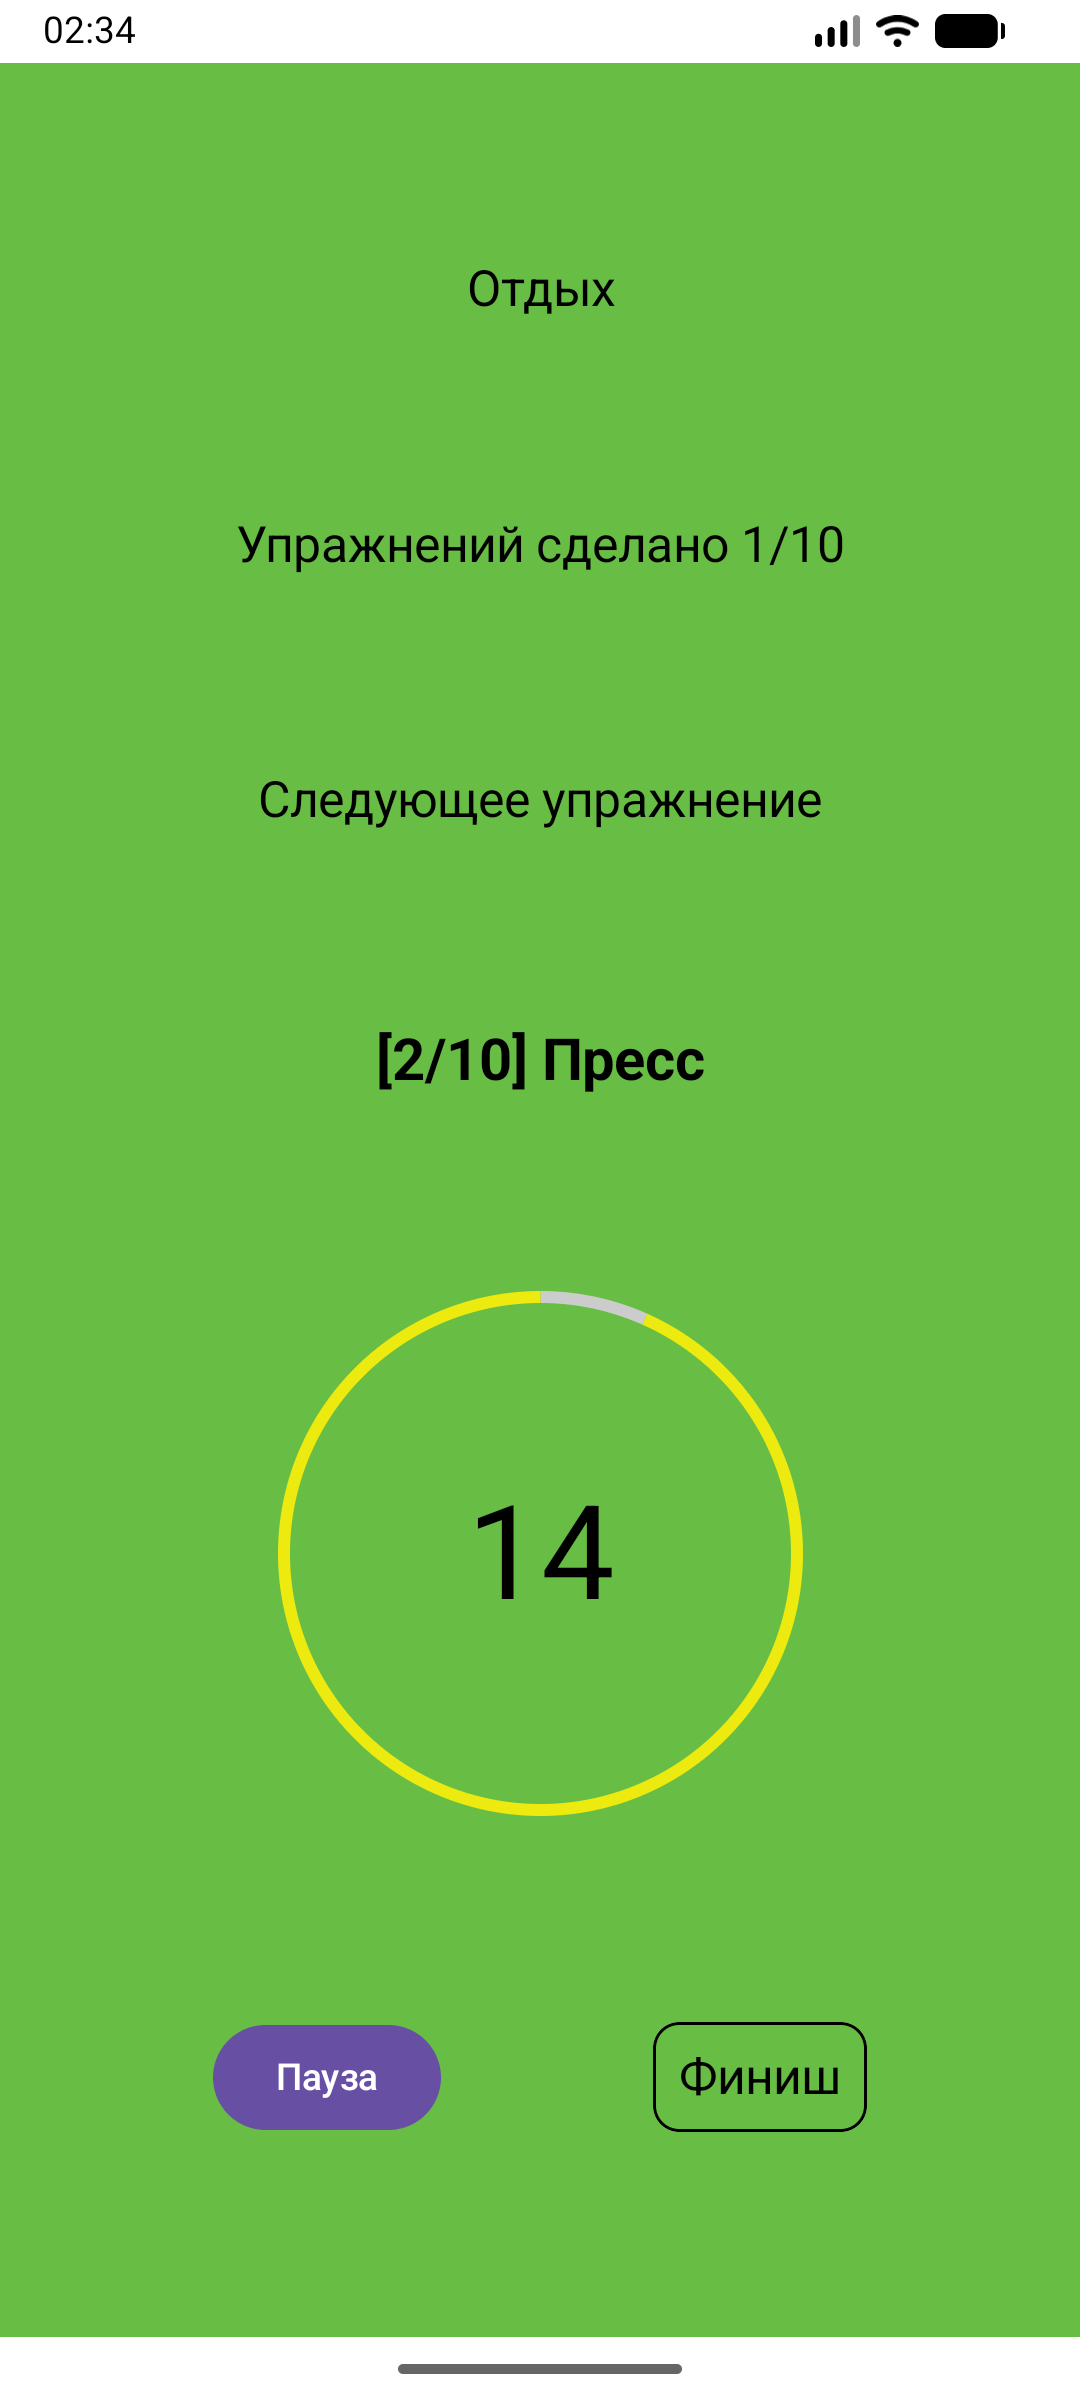
\includegraphics[width=\linewidth]{images/android_screens/rest.png}
        \captionof{figure}{Отдых}
        \label{fig:rest}
    \end{minipage}\hfill
    \begin{minipage}{0.18\textwidth}
        \centering
        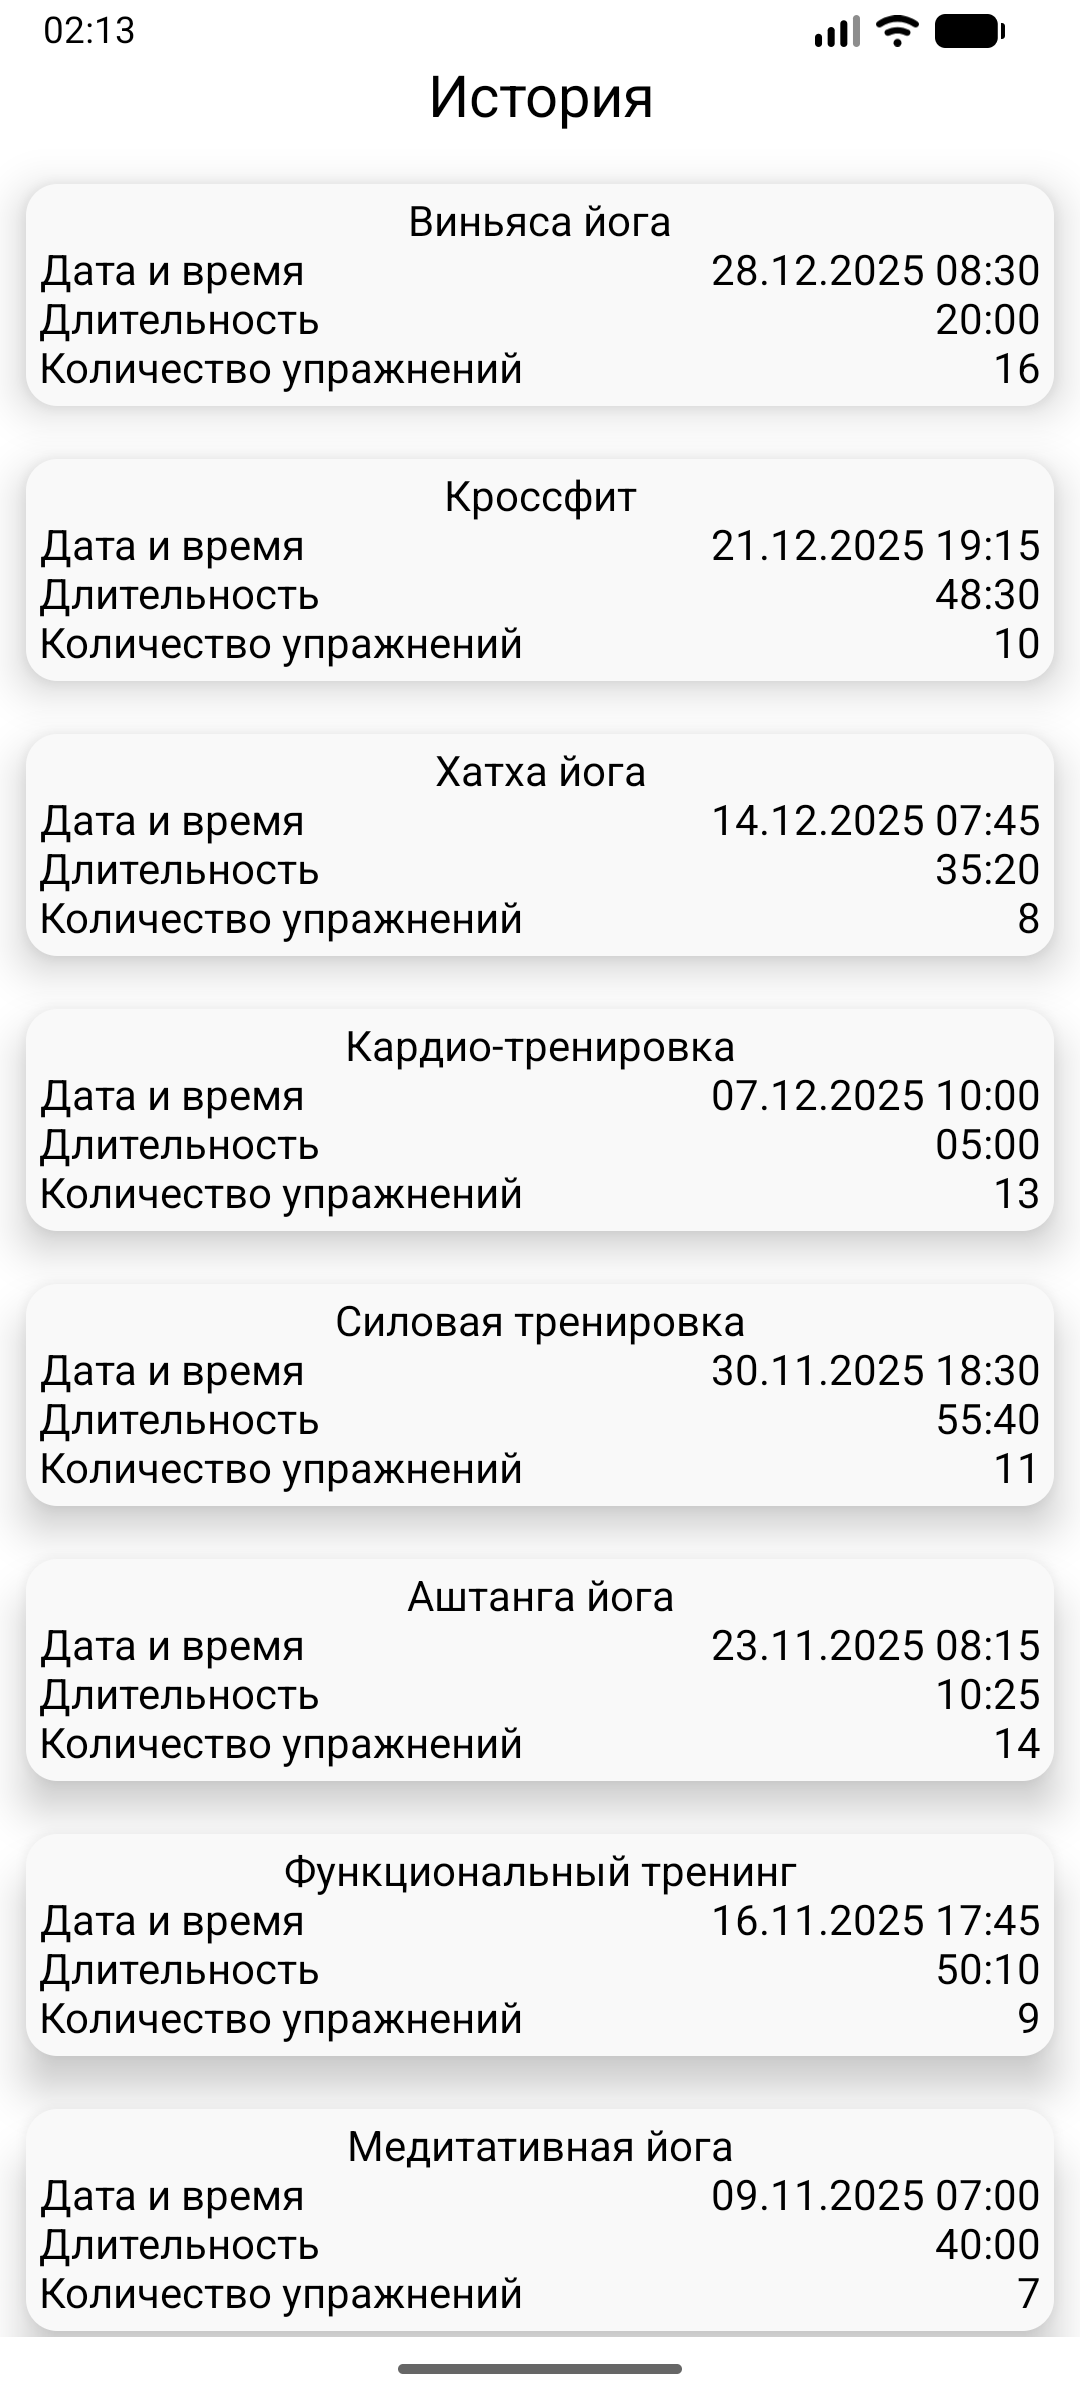
\includegraphics[width=\linewidth]{images/android_screens/history_screen.png}
        \captionof{figure}{История}
        \label{fig:history}
    \end{minipage}\hfill
    \begin{minipage}{0.18\textwidth}
        \centering
        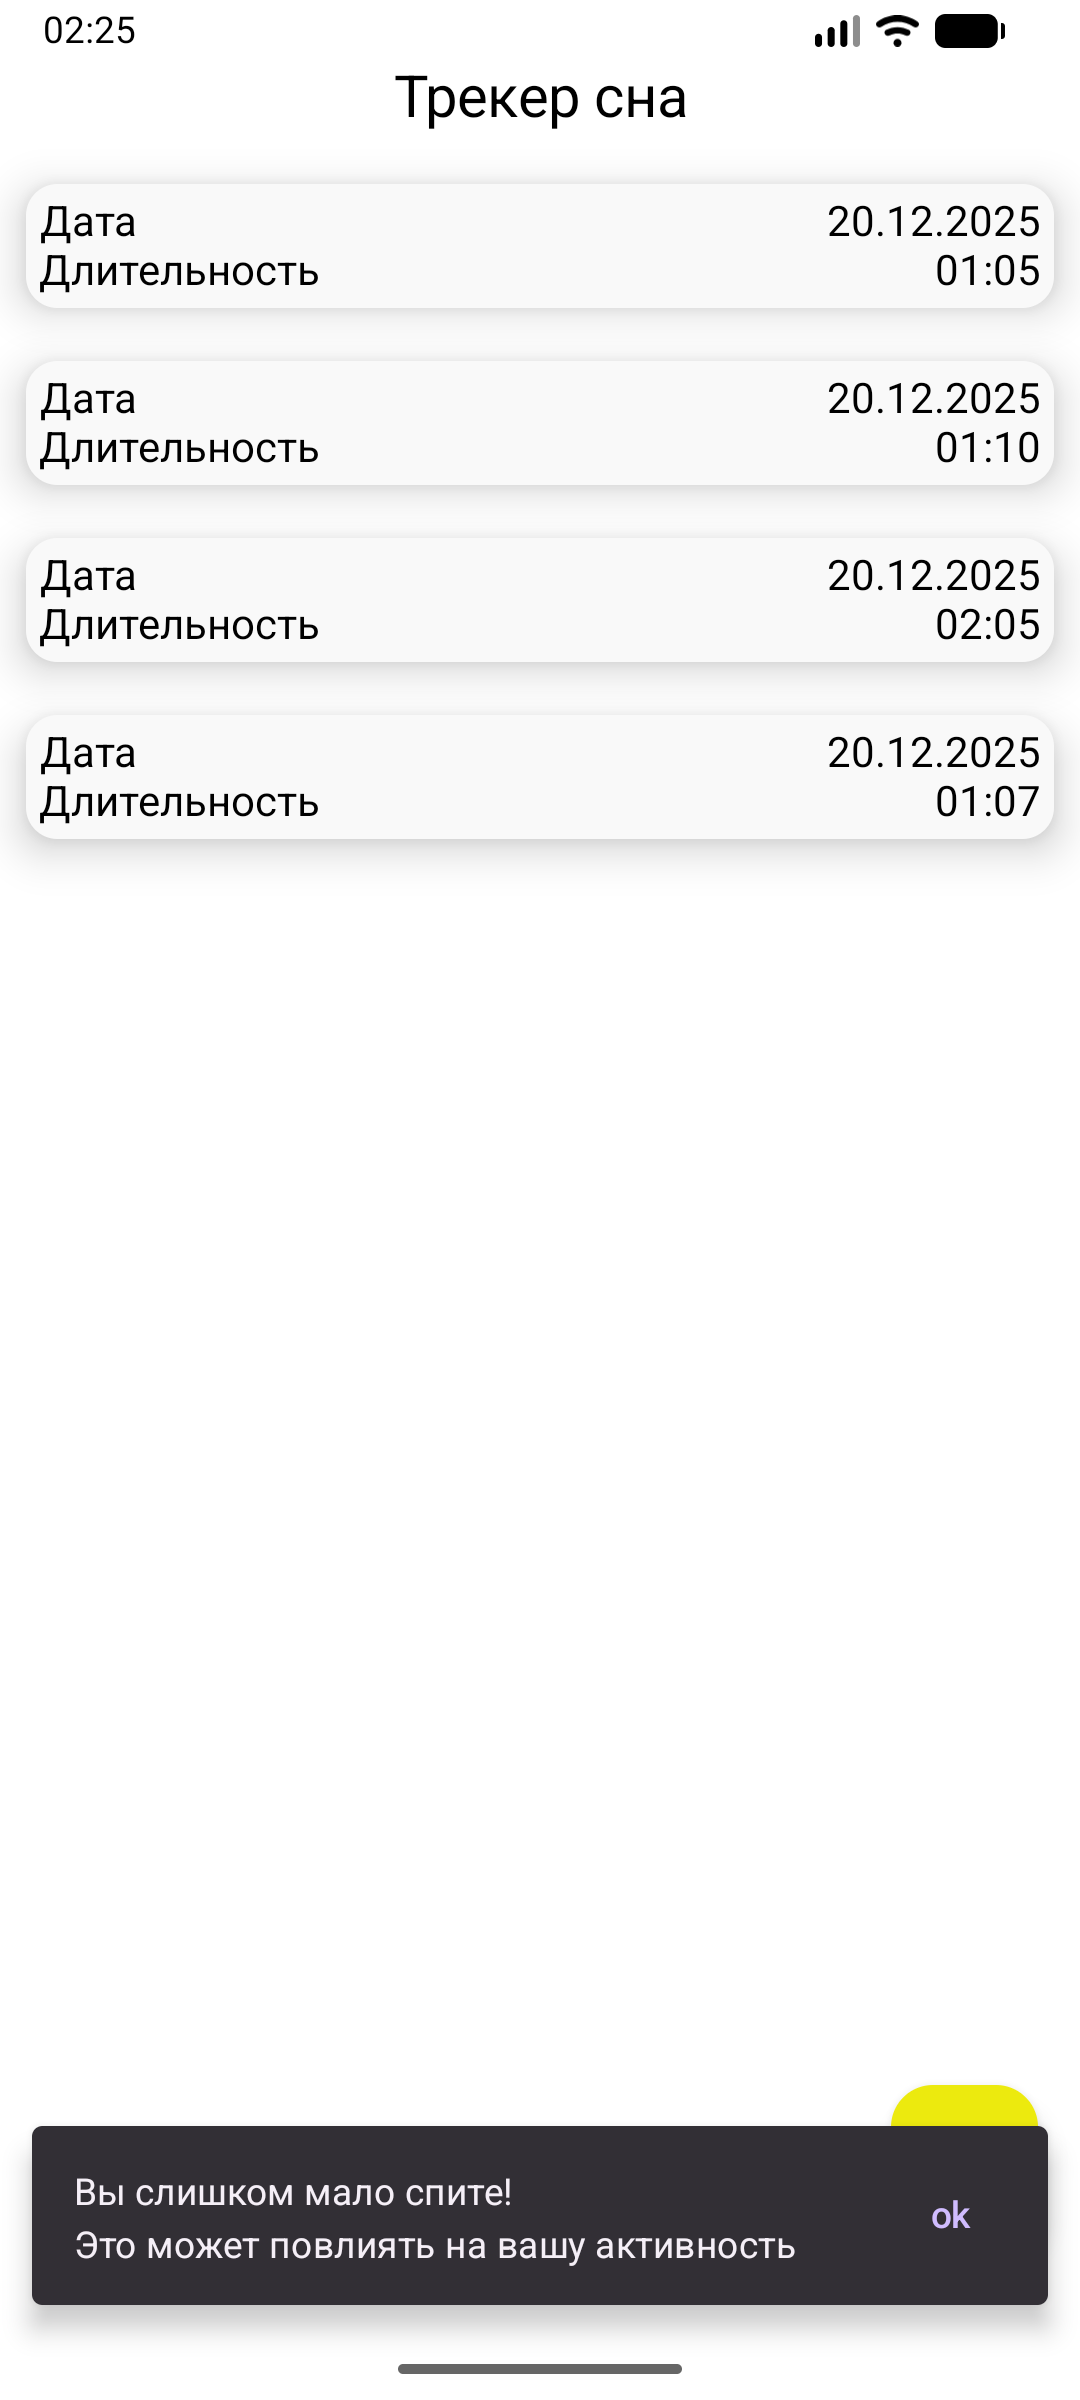
\includegraphics[width=\linewidth]{images/android_screens/sleep_tracker.png}
        \captionof{figure}{Трекер сна}
        \label{fig:sleep}
    \end{minipage}
    \caption*{}
\end{figure}

\subsection{Реализация навигации}
На данном этапе необходимо связать сверстанные экраны в единое приложение. Для реализации логики Bottom Bar будет использоваться Jetpack Navigation. При нажатии на элементы расписания необходимо обеспечить переход на соответствующие детальные экраны или выполнить другие действия, такие как открытие дополнительной информации о занятии. \cite{refh}

На главном экране (рис.~\ref{fig:main}) можно перейти в историю и профиль, нажав на иконку со значками истории и профиля соответственно. Также можно добавить собственную программу тренировок, нажав на иконку добавления (со значком «+»), и перейти к началу уже имеющейся тренировки посредством нажатия на эту тренировку в списке.

На экране входа (рис.~\ref{fig:signin}) нужно ввести имя пользователя зарегистрированного аккаунта и пароль, а после нажать кнопку «Войти» или через кнопку «Нет аккаунта? Зарегистрироваться» перейти на экран регистрации. 

На экране регистрации (рис.~\ref{fig:signup}) нужно ввести имя для регистрации, имя пользователя (username) и пароль, а после нажать кнопку «Зарегистрироваться» или через кнопку «Уже есть аккаунт? Войти» перейти на экран входа. 

На экране тренировки (рис.~\ref{fig:training}) пользователь выполняет упражнения. Выполнение можно поставить на паузу кнопкой «Пауза» с переходом на экран паузы тренировки или «Финиш» с переходом на главный экран. 

На экране профиля (рис.~\ref{fig:profile}) можно увидеть имя и имя пользователя (username) зарегистрированного пользователя, а также с помощью кнопок «Трекер сна» и «Сообщить об ошибке» перейти к экрану трекера сна и открыть почтовое приложение для отправки сообщения об ошибке. 

На экране выбора упражнений перед тренировкой (рис.~\ref{fig:before}) пользователь может добавить или убрать определенные упражнения, скорректировав план тренировки. 

На экране паузы тренировки пользователь может продолжить тренировку, нажав на кнопку «Продолжить».

На экране отдыха пользователь может поставить тренировку на паузу или закончить тренировку нажав на кнопки «Пауза» и «Финиш» соответственно. 

\subsection{Проверка HTTP-запросов}

Для проверки работоспособности разработанного API были выполнены тестовые HTTP-запросы с помощью программы Postman. Каждый запрос сопровождается примером ответа сервера. На рисунках ниже представлены соответствующие скриншоты.

\subsubsection{Регистрация и аутентификация}

На рисунке \ref{fig:register} продемонстрирован запрос регистрации нового пользователя (метод POST, эндпоинт /register). В теле запроса передаются имя пользователя, пароль и отображаемое имя. При успешной регистрации сервер возвращает статус 201 и сообщение.

На рисунке \ref{fig:login} изображён запрос входа в систему (POST /login). После проверки учётных данных сервер выдаёт JWT-токены, которые используются для аутентификации в последующих запросах.

\subsubsection{Управление сном}

На рисунке \ref{fig:sleep_get} показан запрос получения всех записей о сне текущего пользователя (GET /sleep). Запрос требует наличия токена в заголовке Authorization.

На рисунке \ref{fig:sleep_post} представлен запрос добавления новой записи о сне (POST /sleep). В теле передаются дата и продолжительность сна.

На рисунке \ref{fig:sleep_put} приведён запрос обновления существующей записи о сне (PUT /sleep/\{id\}). Идентификатор записи передаётся в пути URL.

На рисунке \ref{fig:sleep_delete} отображён запрос удаления записи о сне (DELETE /sleep/\{id\}).

\subsubsection{Управление упражнениями}

На рисунке \ref{fig:exercises_get} продемонстрирован запрос получения списка всех доступных упражнений (GET /exercises). Список используется при создании тренировок.

На рисунке \ref{fig:exercises_post} показан запрос добавления нового упражнения в справочник (POST /exercises).

\subsubsection{Управление тренировками}

На рисунке \ref{fig:workouts_get} изображён запрос получения всех тренировок с детальным списком упражнений, выполненных в рамках каждой тренировки (GET /workouts).

На рисунке \ref{fig:workouts_post} представлен запрос создания новой тренировки (POST /workouts). В теле передаются дата и время начала, общая длительность и массив упражнений с указанием их идентификаторов и фактической длительности выполнения.

На рисунке \ref{fig:workouts_delete} отображён запрос удаления тренировки по её дате и времени (DELETE /workouts/\{idWorkout\}).

Все приведённые запросы успешно обрабатываются сервером, возвращая ожидаемые коды состояния и данные в формате JSON, что подтверждает корректную реализацию API.

\begin{figure}[H]
	\centering
	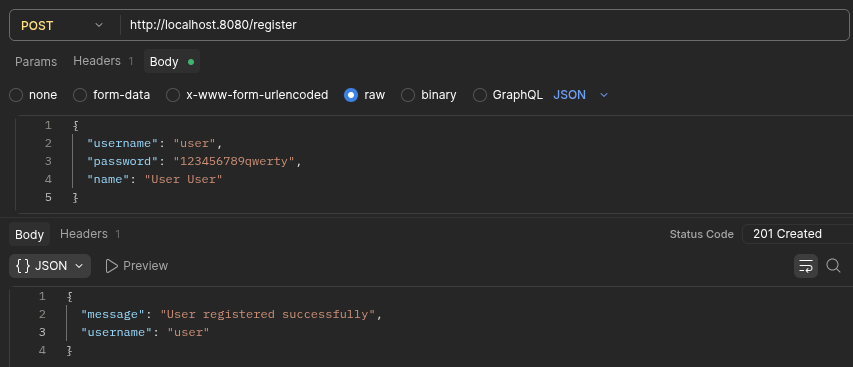
\includegraphics[width=0.8\textwidth]{images/postman/register.png}
	\caption{Запрос регистрации пользователя}
	\label{fig:register}
\end{figure}

\begin{figure}[H]
	\centering
	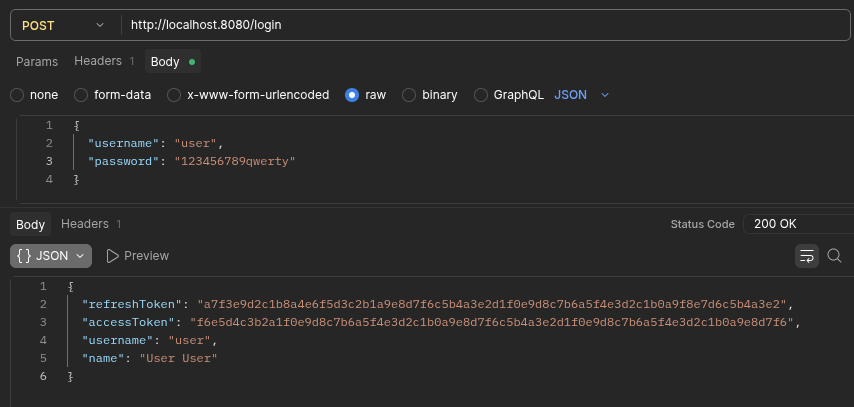
\includegraphics[width=0.8\textwidth]{images/postman/login.png}
	\caption{Запрос входа в систему}
	\label{fig:login}
\end{figure}

\begin{figure}[H]
	\centering
	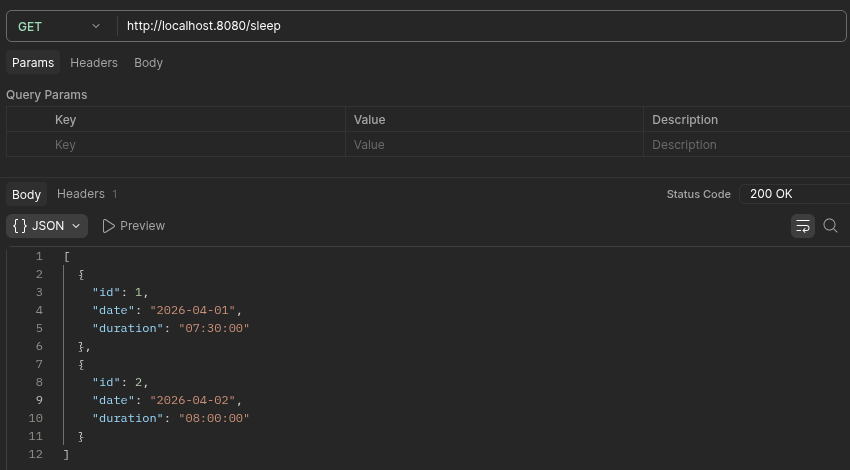
\includegraphics[width=0.8\textwidth]{images/postman/sleep_get.png}
	\caption{Запрос получения записей о сне}
	\label{fig:sleep_get}
\end{figure}

\begin{figure}[H]
	\centering
	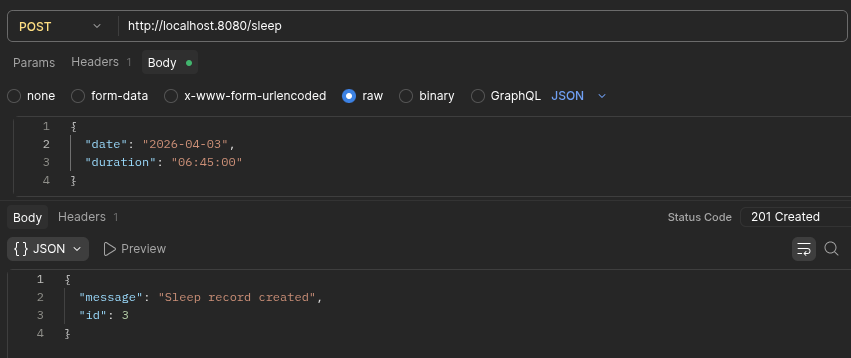
\includegraphics[width=0.8\textwidth]{images/postman/sleep_post.png}
	\caption{Запрос добавления записи о сне}
	\label{fig:sleep_post}
\end{figure}

\begin{figure}[H]
	\centering
	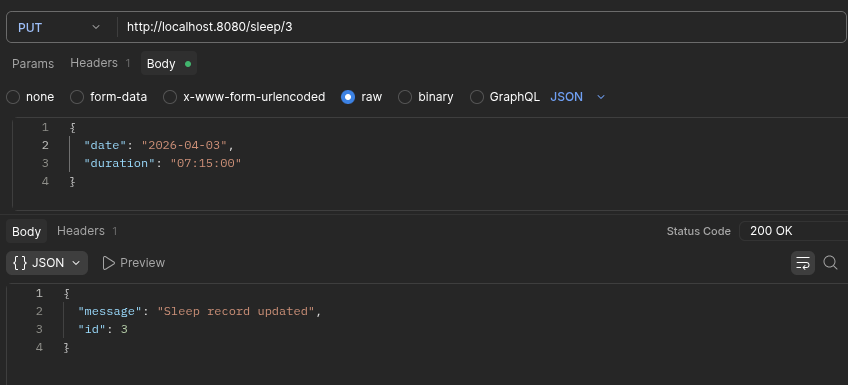
\includegraphics[width=0.8\textwidth]{images/postman/sleep_put.png}
	\caption{Запрос обновления записи о сне}
	\label{fig:sleep_put}
\end{figure}

\begin{figure}[H]
	\centering
	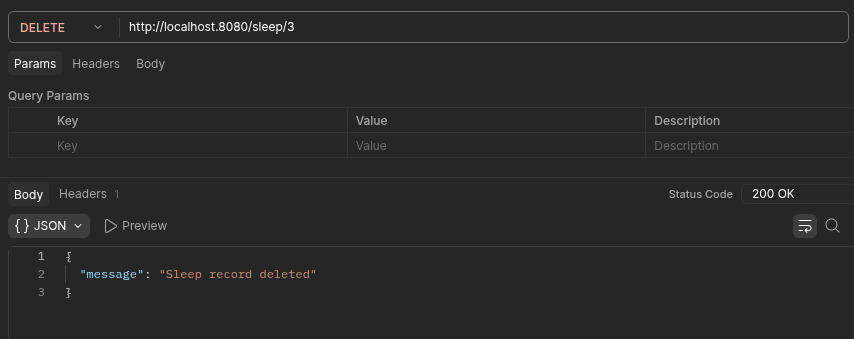
\includegraphics[width=0.8\textwidth]{images/postman/sleep_delete.png}
	\caption{Запрос удаления записи о сне}
	\label{fig:sleep_delete}
\end{figure}

\begin{figure}[H]
	\centering
	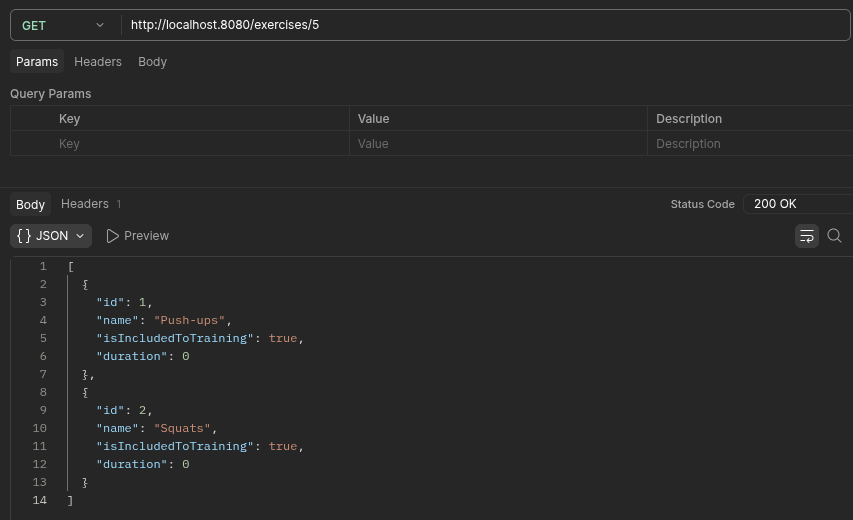
\includegraphics[width=0.8\textwidth]{images/postman/exercises_get.png}
	\caption{Запрос получения списка упражнений}
	\label{fig:exercises_get}
\end{figure}

\begin{figure}[H]
	\centering
	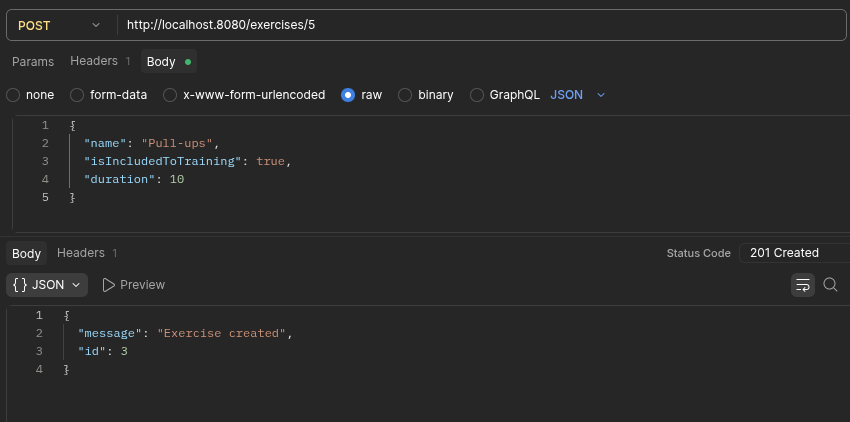
\includegraphics[width=0.8\textwidth]{images/postman/exercises_post.png}
	\caption{Запрос добавления упражнения}
	\label{fig:exercises_post}
\end{figure}

\begin{figure}[H]
	\centering
	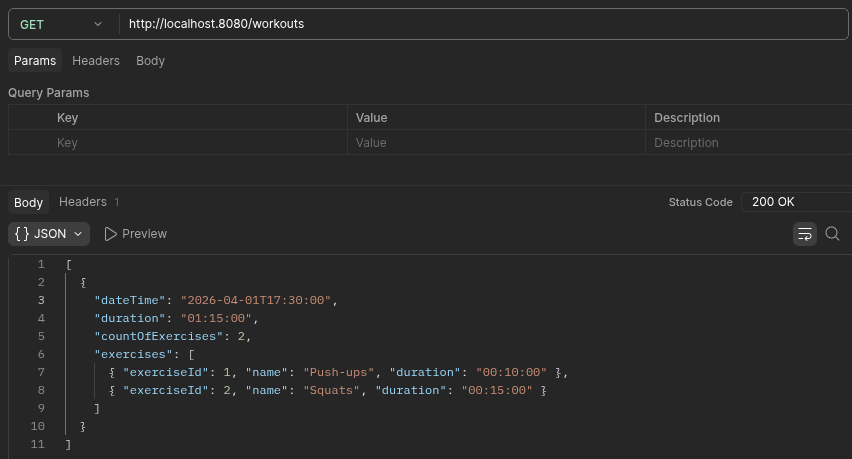
\includegraphics[width=0.8\textwidth]{images/postman/workouts_get.png}
	\caption{Запрос получения тренировок с упражнениями}
	\label{fig:workouts_get}
\end{figure}

\begin{figure}[H]
	\centering
	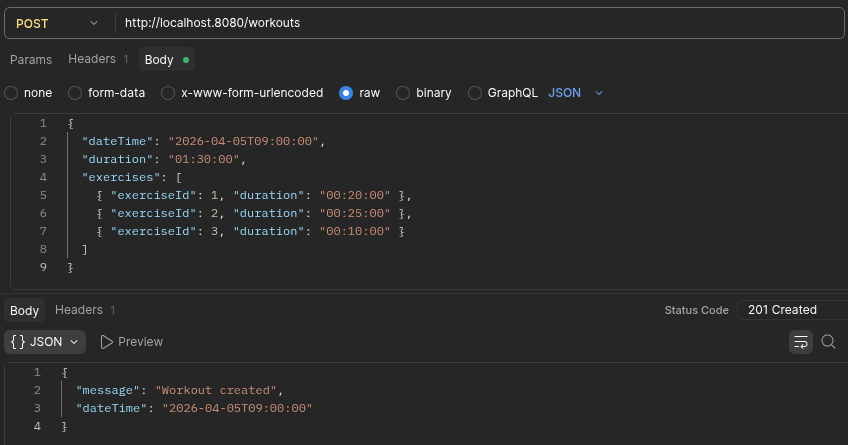
\includegraphics[width=0.8\textwidth]{images/postman/workouts_post.png}
	\caption{Запрос создания тренировки}
	\label{fig:workouts_post}
\end{figure}

\begin{figure}[H]
	\centering
	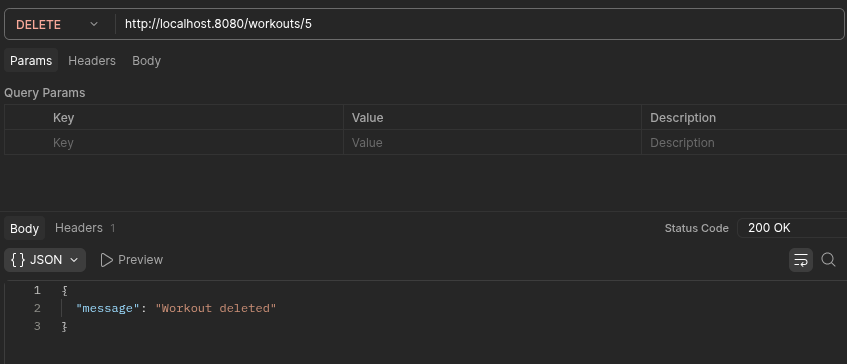
\includegraphics[width=0.8\textwidth]{images/postman/workouts_delete.png}
	\caption{Запрос удаления тренировки}
	\label{fig:workouts_delete}
\end{figure}


\subsection{Логика работы с сетью}

Основная цель работы с сетью — обеспечение взаимодействия приложения с API, для получения информации о расписании по запросу пользователя. \cite{reff}

Для работы с сетью в приложении используются следующие ключевые компоненты, описанные ниже, диаграмма которых изображена на рис. \ref{fig:network_repos}. 
\begin{enumerate}
    \item \textbf{Интерфейсы удалённых репозиториев:}
    \begin{itemize}
        \item \texttt{ExerciseRemoteRepository} — получение упражнений для тренировки.
        \item \texttt{HistoryRemoteRepository} — получение истории занятий и данных учителя.
        \item \texttt{WorkoutRemoteRepository} — получение списка тренировок.
        \item \texttt{SleepRemoteRepository} — получение данных о сне.
        \item \texttt{UserDataRemoteRepository} — регистрация и вход пользователя.
    \end{itemize}
    Каждый интерфейс определяет методы, которые принимают объект запроса и возвращают объект ответа. Это позволяет абстрагироваться от конкретной реализации сетевых вызовов, обеспечивая гибкость и возможность замены реализации (например, для тестирования или смены протокола).

    \item \textbf{Классы-реализации:}
    \begin{itemize}
        \item \texttt{ExerciseRemoteRepositoryImpl},
        \item \texttt{HistoryRemoteRepositoryImpl},
        \item \texttt{WorkoutRemoteRepositoryImpl},
        \item \texttt{SleepRemoteRepositoryImpl},
        \item \texttt{UserDataRemoteRepositoryImpl}.
    \end{itemize}
    Реализуют соответствующие интерфейсы и используют библиотеку \texttt{Retrofit} для выполнения сетевых запросов. Перед отправкой запроса к нему добавляется токен, а также проверяется наличие активного интернет-соединения; при его отсутствии возвращается ответ с кодом ошибки. При успешном выполнении запроса возвращается код 200 и полученные данные. В случае ошибки (отсутствие соединения, неверный запрос и т.п.) возвращаются соответствующие коды ошибок. \cite{refi}

    \item \textbf{Классы DTO (Data Transfer Object):}
    \begin{itemize}
        \item \texttt{ExerciseDTO} — передаёт данные об упражнении: идентификатор упражнения (\texttt{id}), идентификатор тренировки, к которой оно относится (\texttt{idWorkout}), название упражнения (\texttt{name}) и его продолжительность (\texttt{duration}).
        \item \texttt{HistoryDTO} — передаёт данные об истории занятий.
        \item \texttt{WorkoutDTO} — передаёт данные о тренировке
        \item \texttt{SleepDTO} — передаёт данные о сне.
        \item \texttt{UserDataDTO} — передаёт учётные данные пользователя.
    \end{itemize}
    DTO используются для передачи данных между удалённым источником (API) и репозиториями.
\end{enumerate}
\begin{figure}[H]
	\centering
	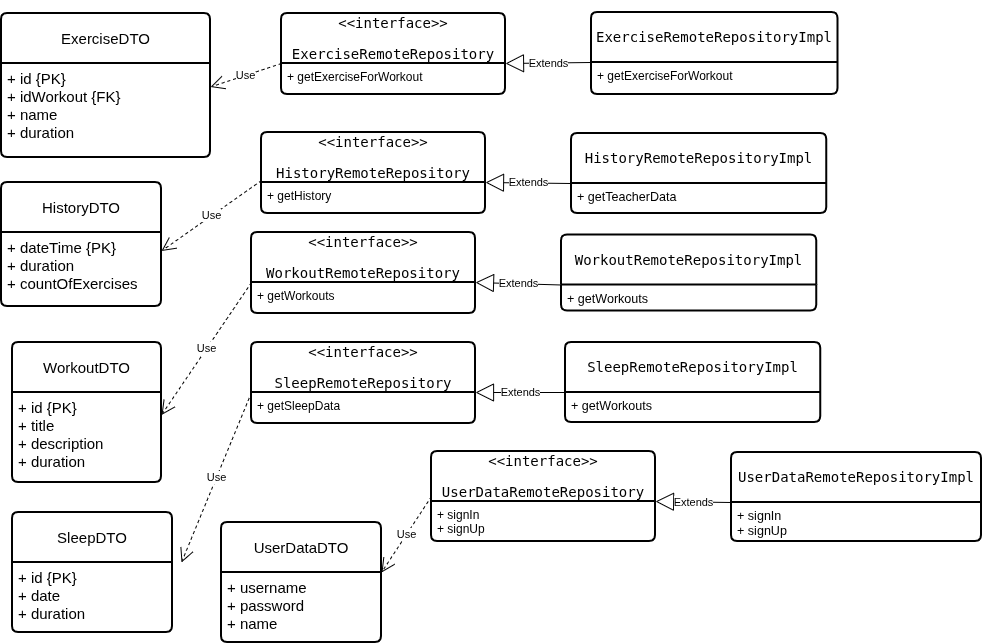
\includegraphics[width=0.8\textwidth]{images/diagrams/Диаграмма классов сетевых репозиториев.png}
	\caption{Диаграмма классов для сетевых репозиториев}
	\label{fig:network_repos}
\end{figure}

\subsection{Логика работы с базой данных}

Для обеспечения надёжного и эффективного хранения данных в приложении используется библиотека Room, которая предоставляет удобный интерфейс для работы с SQLite базой данных в Android-приложениях. Для реализации функциональности работы с базой данных используются следующие основные компоненты.

\begin{enumerate}
    \item \textbf{Entity-классы} представляют собой модели данных, которые будут сохраняться в базе данных. В приложении используются Entity-классы, показанные на схеме базы данных (рис.~\ref{fig:fig8}) и на диаграмме классов (рис.~\ref{fig:database_schema}):
    \begin{itemize}
        \item \texttt{ExerciseEntity} — представляет информацию об упражнении (поля: \texttt{id}, \texttt{idWorkout}, \texttt{name}, \texttt{duration}).
        \item \texttt{HistoryEntity} — представляет информацию об истории занятий (поля: \texttt{dateTime}, \texttt{duration}, \texttt{countOfExercises}).
        \item \texttt{WorkoutEntity} — представляет информацию о тренировке (поля: \texttt{id}, \texttt{title}, \texttt{description}, \texttt{duration}).
        \item \texttt{SleepEntity} — представляет информацию о сне (поля: \texttt{id}, \texttt{date}, \texttt{duration}).
    \end{itemize}
\end{enumerate}

\begin{figure}[H]
    \centering
    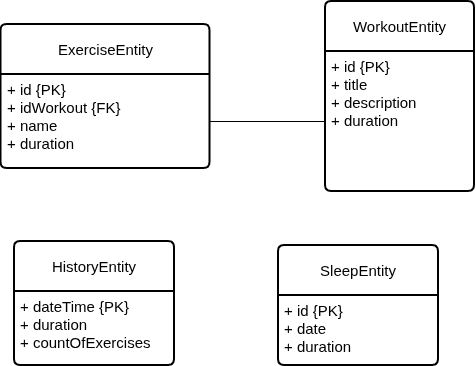
\includegraphics[width=0.8\textwidth]{images/diagrams/Схема бд.png}
    \caption{Схема базы данных}
    \label{fig:fig8}
\end{figure}

\begin{enumerate}[resume]
    \item \textbf{DAO (Data Access Object) интерфейсы} определяют методы для взаимодействия с базой данных. В приложении используются DAO-интерфейсы, изображённые на диаграмме классов (рис.~\ref{fig:database_schema}):
    \begin{itemize}
        \item \texttt{ExerciseDao} — методы для вставки, удаления и получения упражнений.
        \item \texttt{HistoryDao} — методы для вставки, удаления и получения истории занятий.
        \item \texttt{WorkoutDao} — методы для вставки, удаления и получения тренировок.
        \item \texttt{SleepDao} — методы для вставки, удаления и получения данных о сне.
    \end{itemize}
    Эти интерфейсы аннотированы с использованием аннотаций Room: \texttt{@Insert}, \texttt{@Delete}, \texttt{@Query}, которые определяют SQL-запросы, выполняемые для соответствующих операций. \cite{refj}
\end{enumerate}

\begin{figure}[H]
    \centering
    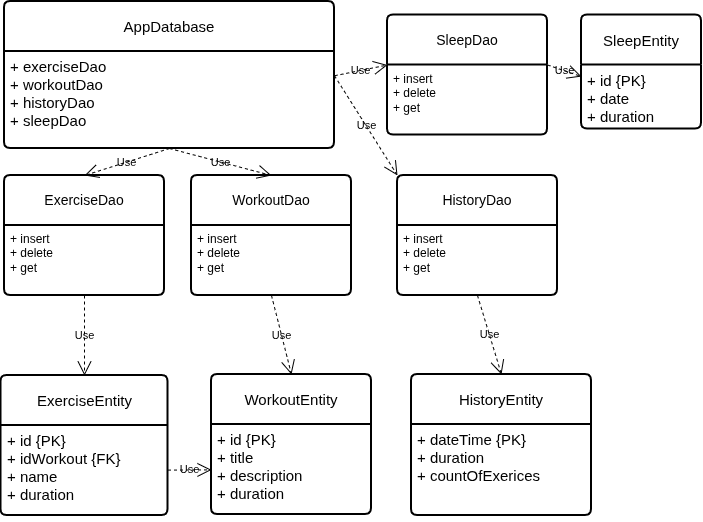
\includegraphics[width=0.8\textwidth]{images/diagrams/Диаграмма классов бд.png}
    \caption{Диаграмма классов базы данных}
    \label{fig:database_schema}
\end{figure}

\begin{enumerate}[resume]
    \item \textbf{Абстрактный класс базы данных} наследуется от \texttt{RoomDatabase} и служит точкой входа для взаимодействия с БД. В приложении определён класс \texttt{AppDatabase} (рис.~\ref{fig:database_schema}), который содержит абстрактные методы, возвращающие экземпляры DAO:
    \begin{itemize}
        \item \texttt{abstract fun exerciseDao(): ExerciseDao}
        \item \texttt{abstract fun historyDao(): HistoryDao}
        \item \texttt{abstract fun workoutDao(): WorkoutDao}
        \item \texttt{abstract fun sleepDao(): SleepDao}
    \end{itemize}

    \item \textbf{Клиент базы данных} предоставляет методы для взаимодействия с БД через DAO. Room автоматически генерирует реализацию \texttt{AppDatabase\_Impl} (на основе аннотаций), которая инкапсулирует логику работы с SQLite. Другие компоненты приложения получают экземпляр \texttt{AppDatabase} (например, через синглтон или инъекцию зависимостей) и вызывают методы DAO для выполнения CRUD-операций. Это обеспечивает удобный интерфейс и изолирует детали работы с базой данных от остального кода.
\end{enumerate}


\subsection{Архитектура приложения}

Приложение разработано с соблюдением принципов чистой архитектуры~\cite{refd}, что обеспечивает высокую степень модульности, гибкости, тестируемости кода, а также упрощает поддержку и расширение функциональности \cite{refc}. Чистая архитектура разделяет систему на несколько слоёв, каждый из которых имеет чётко определённые задачи и зависимости (рис.~\ref{fig:clean_arch}):

\begin{figure}[H]
    \centering
    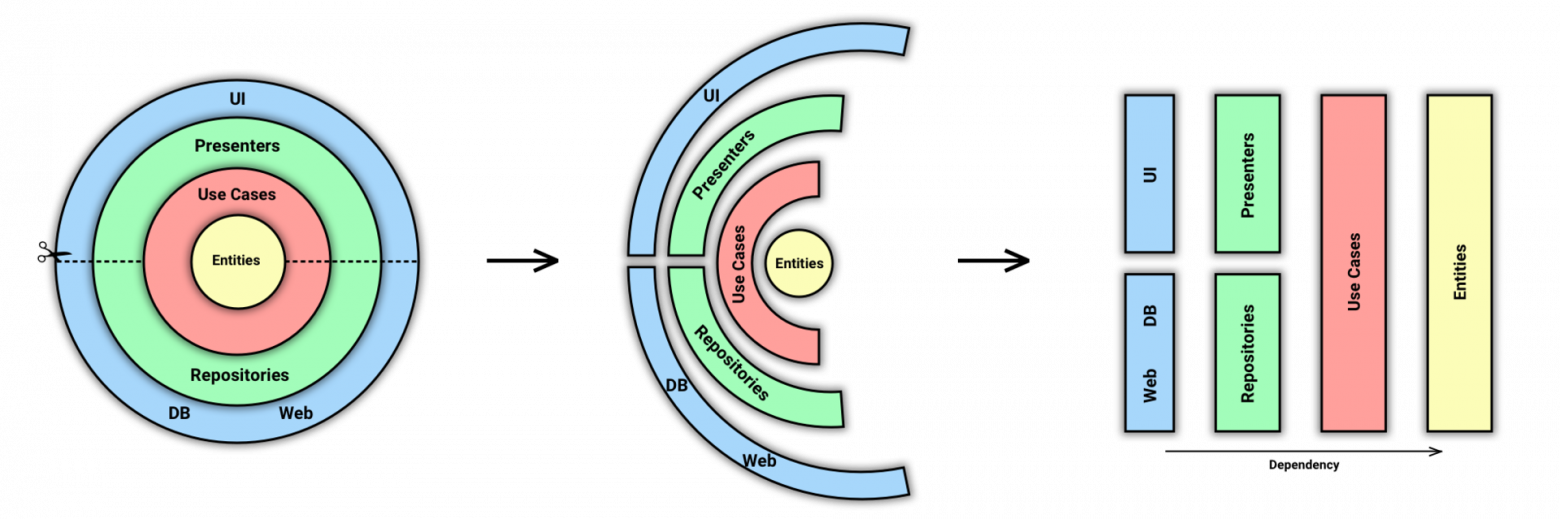
\includegraphics[width=0.8\textwidth]{images/diagrams/слои чистой архитектуры.png}
    \caption{Слои чистой архитектуры}
    \label{fig:clean_arch}
\end{figure}

\begin{enumerate}
    \item \textbf{Внешний слой (UI Layer)}: включает все компоненты, связанные с пользовательским интерфейсом, такие как фрагменты и активности. Основная задача UI Layer — отображение данных и взаимодействие с пользователем. Этот слой получает данные из ViewModel и обновляет интерфейс в соответствии с изменениями в данных \cite{refc}.
    \item \textbf{Слой данных (Data Layer)}: содержит компоненты, связанные с управлением данными, включая DAO-интерфейсы для работы с Room, реализации сетевых запросов с использованием Retrofit, а также клиентов базы данных и сетевых клиентов. Data Layer отвечает за получение и хранение данных, предоставляя их в Domain Layer через репозитории \cite{refc}.
    \item \textbf{Слой домена (Domain Layer)}: содержит бизнес-логику и бизнес-модели. Domain Layer не зависит от других слоев и содержит основные бизнес-правила и интерфейсы репозиториев \cite{refc}.
    \item \textbf{Слой приложений (Application Layer)}: содержит ViewModel, которые объединяют бизнес-логику с логикой представления и управления состоянием. ViewModel взаимодействуют с репозиториями для получения данных и обработки пользовательских действий.
\end{enumerate}

Для разделения представления и логики управления данными в приложении используется паттерн MVVM (Model-View-ViewModel)~\cite{refe}. Этот паттерн (рис.~\ref{fig:mvvm}) обеспечивает чёткое разделение обязанностей между компонентами приложения:

\begin{figure}[H]
    \centering
    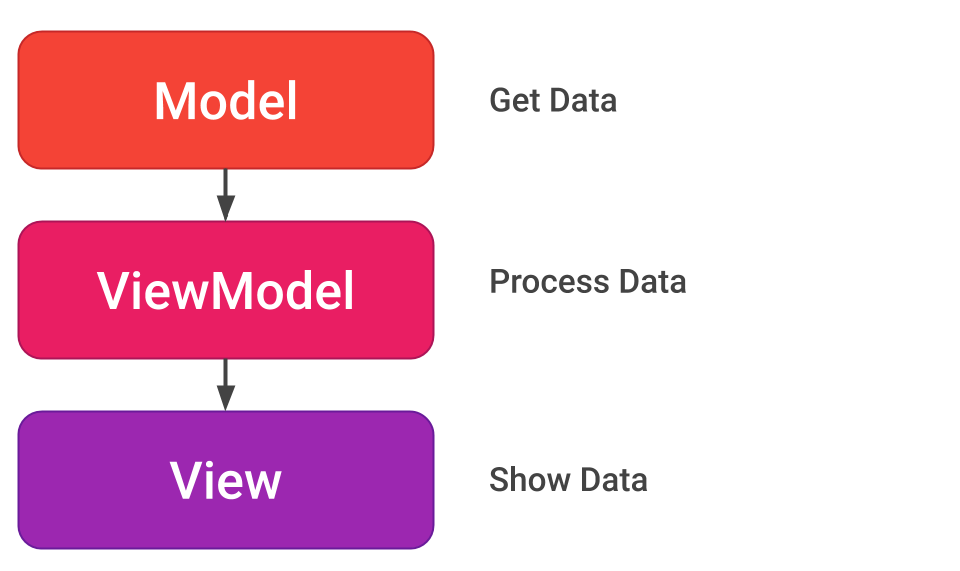
\includegraphics[width=0.8\textwidth]{images/diagrams/компоненты mvvm.png}
    \caption{Компоненты паттерна MVVM}
    \label{fig:mvvm}
\end{figure}

\begin{enumerate}
    \item \textbf{Model}: включает бизнес-логику и данные приложения. Модель получает данные из Data Layer и предоставляет их ViewModel.
    \item \textbf{View}: состоит из пользовательского интерфейса и отвечает за отображение данных. View наблюдает за изменениями в ViewModel и обновляет интерфейс в соответствии с этими изменениями.
    \item \textbf{ViewModel}: посредник между View и Model. ViewModel запрашивает данные у Model и предоставляет их View, а также обрабатывает пользовательские действия и обновляет Model.
\end{enumerate}

Для управления зависимостями и их внедрения в приложении используется библиотека Koin. В модулях Koin определяются зависимости и способы их создания. Например, можно определить зависимости для сетевого клиента, базы данных и ViewModel. Это позволяет централизованно управлять зависимостями и облегчает их модификацию. Koin автоматически предоставляет экземпляры классов, когда они требуются, что упрощает тестирование и модульность. Например, ViewModel могут получать необходимые репозитории через Koin, что устраняет жёсткие зависимости \cite{refj}.
